\documentclass[a4paper]{article}
\usepackage[T1]{fontenc}
\usepackage{filecontents}
\usepackage[utf8]{inputenc}
\usepackage{verbatim}
\usepackage{hyperref}
%\usepackage{pdfpages}
\usepackage{graphicx}
\graphicspath{{plot/kinematic/}}
\graphicspath{{plot/optimization/}}
\usepackage{subfigure}
\usepackage{tikz, amsmath}
\usepackage[font=footnotesize]{caption}
\usepackage{amsmath,amsfonts,bm} 
\usepackage{caption}
\usepackage{float}
\usepackage{geometry}
\usepackage{multirow}
\usetikzlibrary{shapes, positioning, arrows}
\graphicspath{ {} }
\title{Biped Walking Pattern Generation based on Spatial Quantized Dynamics}
\author{Dario Zurlo}
\date{01 April 2021} 


\begin{document}
\maketitle

\newpage

\section{Introduction}

Control a bipedal robot locomotion is a challenging task due to complexity of the system that needs to maintain constantly the balance on its two legs during the walking, many techniques has been studied in the past to generate static and dynamic biped gait on flat and rough terrain. First kind of locomotion developed is static walking, i.e. locomotion in which the robot moves slowly. The reason why this kind of locomotion was the first implemented, is because the joint actuators were big and the computation power was poor. The second one is the dynamic walking that is the non static locomotion where the walking speed is higher. Nowadays the latter can be implemented on a robot more easily thank to the smaller joint actuators and the high computation power. This great computational power has opened the way for other control techniques, some of them are no more based on the kinematic model of the robot such as reinforcement learning techniques or in general techniques based on artificial intelligence, and other are based on optimal control in which the aim is to determine the control law, that applied to the system optimizes its operation with respect to some pre-estabilished evaluation criteria, always taking into account the limit of the system. The latter is the one  which the project is based on.

\section{Problem Definition}

The aim of this project is to reproduce some of the results of bipedal gait generation based on Zero Moment Point (ZMP) with a novel system modeling, named Spatially Quantized Dynamics (SQD) introduced in \cite{Kaj1} and show how this technique is more flexible with respect to the classic one, based on time quantization, in order to allow the robot to walk with stretched knees.\\
The notion of ZMP has never been introduced by a formal definition \cite{Vukobratovic}, the notion that we are going to use is that the ZMP is the point with respect to which the moment of the contact force is zero in the horizontal direction.
The analysis is performed by considering only horizontal and flat ground both in the sagittal and coronal plane, without considering any obstacle during the walking, this is an enormous simplification but the reason why we do all these simplifications is because we want to show why this technique is suitable in the case of stretched knees.\\
The ZMP based gait generation is a widely known in the area of walking robot in which the aim is to design a ZMP trajectory such that it always lies in the support polygon (SP), that is a sufficient condition for dynamical balance; this is done by taking the CoM trajectory such that the ZMP moves as planned. The steps followed to design the ZMP based gait are, first of all, design the steps sequence and the relative SP, then design the ZMP reference that it is always inside the SP and then compute the CoM trajectory such that the  ZMP moves as planned. Once the CoM trajectory is available then it is possible to move the legs such that the CoM and the steps move as planned. The steps illustrated are independent of the model used, the common one discretized with respect to time or the one discretized with respect to space.\\
The first problem that arises is due to the complexity of the full humanoid dynamics necessary to  directly control the ZMP, for this reason the control of the ZMP is done by controlling the CoM trajectory, that is easier, because it is possible to use a simple linear model called Linear Inverted Pendulum (LIP), that relates the evolution of the CoM, that is the output, with the evolution of the ZMP, that is the input. Where the CoM can be varied by changing the robot configuration through its joints. The dual model is the Cart Table model (CT) suitable to track the ZMP, that in this case is the output and the CoM is the input.\\
The novelty introduced in the paper on which this project is based on, is in the way in which the dynamics of our robot is discretized. In fact, instead of discretizing the model with respect to time as usual, the model is discretized with respect to the space. This renders the problem more difficult to treat, as we will see later, but the advantage is that it is possible to realize versatile gait generation.\\
To solve this problem it has been used nonlinear optimization techniques; differently form the paper, I  optimized the cost index on the full horizon using the standard Matlab function, instead of using the  the Matlab toolbox of Differential Dynamic Programming (DDP) developed by Tassa, Mansard and Todorov \cite{Tassa} as the authors did in \cite{  Kaj1}.  The results are the same, the difference is in the computation time.\\
The last step, once the CoM of the robot is computed, is to generate an array of vectors containing all the configurations of the joints; in order to achieve this task it is necessary to compute the inverse kinematics numerically, since the closed form solution can be difficult to find and also because we want to obtain a robust solution against kinematic singularities. The technique used in \cite{Kaj1} is the inverse kinematics based on Levenberg-Marquardt method with robust damping \cite{LMmethod}, because they want also deal with stretched knees that is a singular configuration of the robot legs. We want also to deal with this latter problem firstly comparing three different numeric inverse kinematics techniques and at the end choosing the the best method.\\
Once the array of configuration is complete, to implement the the walking on the real robot it is necessary to perform a conversion form space domain into time domain. I will give just an idea on how to perform this conversion.  


\section{Gait Generation based on ZMP}


The term gait is used to indicate a sequence of leg and body motions, that propels the robot along some path. In this project we want to study a particular gait generation based on ZMP. In order to find the point with respect to which the moment of the contact forces is zero,i.e. the ZMP, we consider the Euler's rotation equation, that describes the rotation of a rigid body.

\begin{equation}
(\pmb{c}-\pmb{o})\times M \ddot{\pmb{c}}+\dot{\pmb{L}} = \sum_i{(\pmb{p_i}-\pmb{o})}\times \pmb{f_i}-(\pmb{c}-\pmb{o})\times M\pmb{g}
\label{eq:eulereq}
\end{equation}   

Where $\pmb{c}$ is the position of the CoM, $\pmb{o}$ is the generic position with respect to which we want to compute the moment, $M$ is the total mass of the robot, $\pmb{L}$ is the angular momentum of the robot with respect to its CoM given by the sum of the angular momentum of each robot link, $\pmb{f}_i$ is the force applied at point $\pmb{p_i}$, that is the contact point, and $\pmb{g}$ is the gravitational acceleration.\\
We now consider the torque around the ZMP given by

\begin{equation}
\pmb{\tau} = \sum_i{(\pmb{p_i}-\pmb{z})}\times \pmb{f_i}
\label{eq:zmpcond}
\end{equation} 

That written in terms of vector components  is 

\begin{equation}
\pmb{\tau}_x = \sum_i{(p_{iy}-z_y)}f_{iz}-\sum_i{(p_{iz}-z_z)}f_{iy}
\label{eq:zmpx}
\end{equation} 

\begin{equation}
\pmb{\tau}_y = \sum_i{(p_{iz}-z_z)}f_{ix}-\sum_i{(p_{ix}-z_x)}f_{iz}
\label{eq:zmpy}
\end{equation} 

\begin{equation}
\pmb{\tau}_z = \sum_i{(p_{ix}-z_x)}f_{iy}-\sum_i{(p_{iy}-z_y)}f_{ix}
\label{eq:zmpz}
\end{equation} 

the position of the ZMP can be obtained by settling \eqref{eq:zmpx} and \eqref{eq:zmpy} to zero. In fact in case of horizontal and flat plane, all the contact point along the $z$ axis are the same and are also equal to the $z$ component of the ZMP, then the second term of \eqref{eq:zmpx} and the first term of \eqref{eq:zmpy} become zero. This yields

\begin{equation}
\pmb{z} = \frac{\sum_i{\pmb{p_i}f_i}}{\sum_if_i}
\label{eq:zmppoint}
\end{equation} 

that is the point that we are looking for, under the assumption that the ground is flat and horizontal. The third component of \eqref{eq:zmpcond} is in general different from zero, this means that there is torque due to the friction between the foot and the ground.

Now using the definition of the ZMP to guarantee the dynamical balance during walking, we need that the ZMP is at every instant inside the SP, that continuously changes during walking according to the cyclic alternation of 4 phases , if the robot is able to rotate the feet or 2 phases if the robot walks with flat feet.

\begin{comment}
Now using the definition of the ZMP to guarantee the dynamical balance during walking, we need that the ZMP is at every instant inside the SP, that continuously changes during walking. According to the cyclic alternation of four phases of each leg, if the robot is able to rotate the feet, we have all four phases, whereas if the robot walks with flat feet we will have two phases. 
\end{comment}

In this project I consider that the robot is able to rotate its feet and then I consider all the four phases during walking. In figure \ref{fig:SPZMPsagittal} and \ref{fig:SPZMPcoronal} are shown the SP and the desired ZMP respectively along the sagittal axis and along the coronal axis. 

\begin{figure}
     \begin{minipage}[b]{0.48\textwidth}
         \centering
         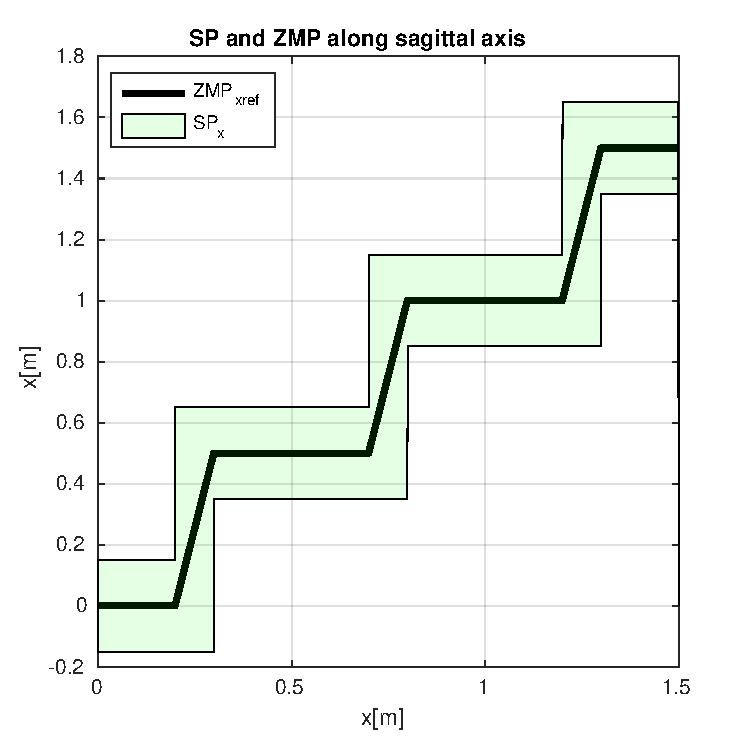
\includegraphics[width=\textwidth]{plot/optimization/SPx.pdf}
         \caption{SP and desired ZMP along sagittal axis}
         \label{fig:SPZMPsagittal}
     \end{minipage}
     \hfill
     \begin{minipage}[b]{0.48\textwidth}
         \centering
         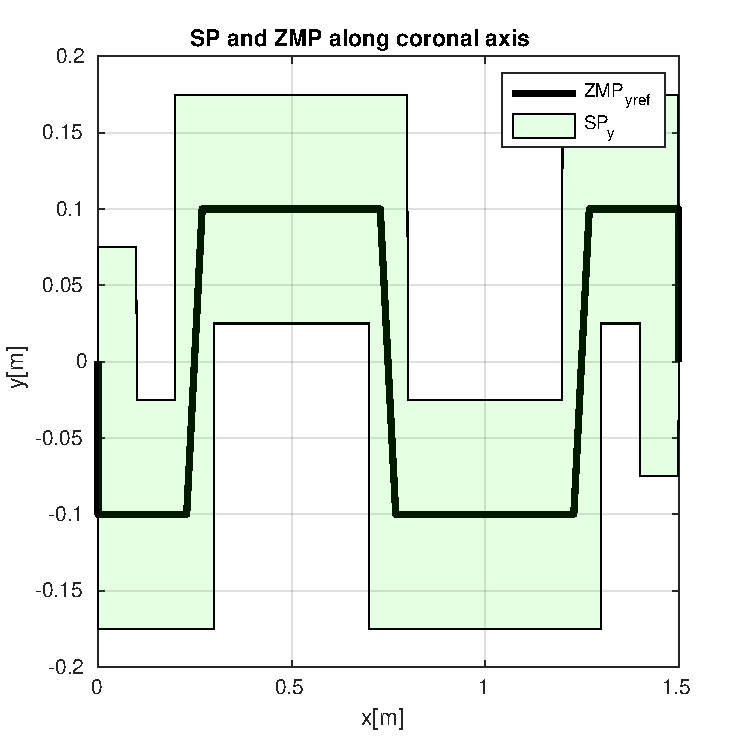
\includegraphics[width=\textwidth]{plot/optimization/SPy.pdf}
         \caption{SP and desired ZMP along coronal axis}
         \label{fig:SPZMPcoronal}
     \end{minipage}       
\end{figure}

It is clear that the first step is to define a set of robot steps as shown in the figure \ref{fig:footsteps}, through the foot steps planner, in order to define the SP. Once I have the support polygon, I design a suitable ZMP trajectory that is given as a reference of the optimization problem. The result of the optimization problem is the position of the ZMP and also the position of the CoM that makes the ZMP trajectory moves as I planned. 

\begin{figure}
 \centering
 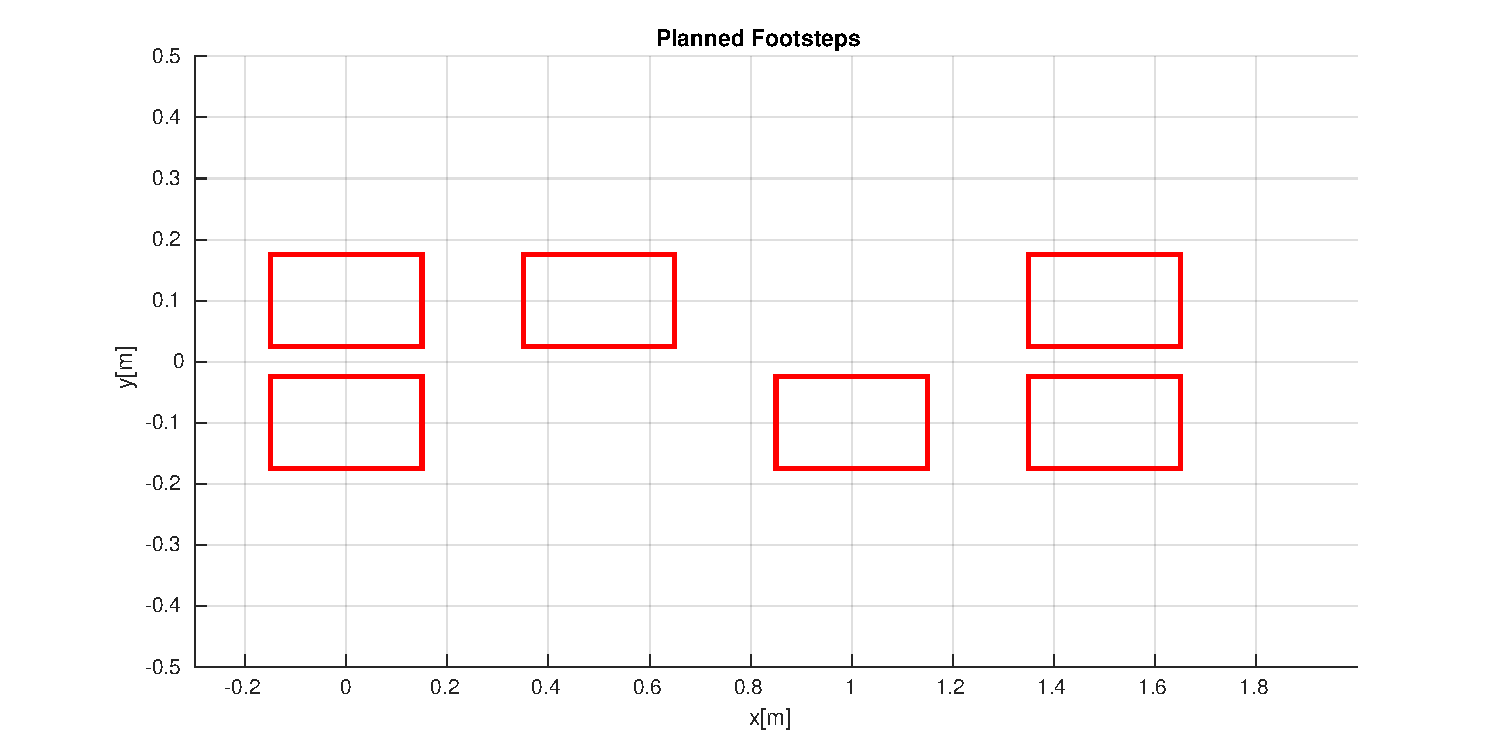
\includegraphics[width=\textwidth]{plot/optimization/footsteps.pdf}
 \caption{Three footsteps planned}
 \label{fig:footsteps}
\end{figure}

\section{Dynamical Model}
%speigare LIP CT l'estensione e schema a blocchi 

A full dynamical model of a humanoid robot with many DoF can be very difficult to obtain and above all it can hide the balance of the robot, then a simplified version of the model, that is enough accurate to describe the balance, is necessary. 
A possible approach, under the assumption that all the mass of robot is concentrated at the CoM and that the robot has massless legs, is to approximate the dynamics of the robot with the dynamics of an inverted pendulum with variable length,  as shown in figure \ref{fig:LIPM}. Using the Euler-Lagrangian formulation it is possible to obtain the following model for the inverted pendulum

\begin{equation}
\begin{aligned}
r\ddot{\theta}+2r\dot{r}\dot{\theta}-grsin(\theta)=\tau/M\\
\ddot{r}-r\dot{\theta}^2+gcos(\theta) = f/M
\end{aligned}
\end{equation}

Where $g$ is the gravity acceleration, $M$ is the total mass of the robot, $r$ is the length of the pendulum, $\theta$ is the angle of inclination with respect to the vertical, $f$ is the force at the prismatic joint along the length and $\tau$ is the torque at the pivot, that in general is small and in case of dimensionless foot is zero. The idea to move the CoM along the longitudinal direction is to apply a force $f$ to compensate the gravity, this force is given by the following equation

\begin{equation}
    f = \frac{Mg}{cos(\theta)}
\end{equation}

Then the longitudinal evolution of the CoM is given by

\begin{equation}
    M\ddot{c}^x=Mgtan(\theta)=Mg\frac{c^x}{c^z}
    \label{eq:long_ev_x}
\end{equation}

Where $\pmb{c}$ is the CoM position and the apex indicate the component of the vector $x$, $y$ or $z$. 

\begin{comment}
The most used model is the Linear Inverted Pendulum model (LIP), that describes quite well the relationship between the evolution of the CoM and the evolution of the ZMP, and it is linear hence is more suitable for controller synthesis.
In general the model of a pendulum is nonlinear, in fact there is a trigonometric non-linearity, as it is possible to see in \ref{eq:invpend}, where $\theta$ is the angle of inclination with respect to the vertical, $r$ is the length of the pendulum and $g$ is gravity acceleration. 

\begin{equation}
\ddot{\theta} = \frac{g}{r}sin(\theta)
\label{eq:invpend}
\end{equation} 

However if we reasonably assume that the height of the CoM of the robot is kept constant, in fact the robot moves on a horizontal flat ground  and we can consider the height of the CoM as the average of the height during the whole walking, then the pendulum model became linear as it is possible to see from the following equation

\begin{equation}
\ddot{c} = \frac{g}{z}c
\label{eq:linearinvpend}
\end{equation} 

where $c$ is the position of the CoM and $z$ is the height of the CoM.

%However if we reasonably assume that the height of the CoM of the robot is kept constant, since we are considering the walking on %horizontal flat ground, and we can take as the height the average of the CoM height, we can define the LIP model.
%As a consequence the inverted pendulum model becomes linear, as it is possible to see from \ref{eq:linearinvpend}, where $c$ is the position of the CoM and $z$ is the height of the CoM.
\end{comment}


It is possible to obtain a similar model as \eqref{eq:long_ev_x} from eq (\ref{eq:eulereq}) dividing by the forces along the $z$-axis and neglecting the variation of the angular momentum $\dot{L}$, that is the variation of the angular momentum of each joint;
%due to the variation of the angular momentum of each joint 
in this way we obtain the LIP model
\begin{equation}
\ddot{\pmb{c}}^{x,y} = \frac{g^z}{c^z}(\pmb{c}^{x,y}-z^{x,y})
\label{eq:LIPM}
\end{equation}
Where $z^{x,y}$ is the ZMP position along the axis $x$ or $y$, that push away the CoM position and is the input of the model . 




\begin{figure}
 \centering
 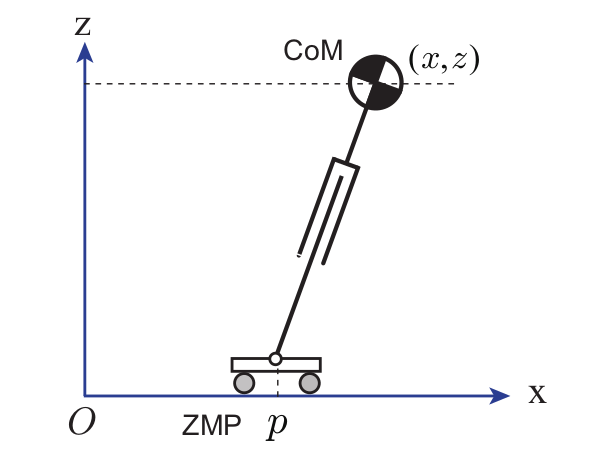
\includegraphics[width=0.5\textwidth]{plot/dynamics/LIP.png}
 \caption{LIP model}
 \label{fig:LIPM}
\end{figure}

Since the CoM position along the $x$ axis has a good correspondence with the horizontal hip displacement, we can expect that the robot dynamics can be expressed by the linear inverted pendulum model in which $x$ represent both the hip position and the CoM position. Instead the CoM position along the $z$ axis in the actual robot is not constant but we can assume it as the average of the CoM height during the whole walking.
For simplicity I analyze, first of all, the problem along the sagittal axis and the equation (\ref{eq:LIPM}) becomes  
\begin{equation}
\begin{aligned}
\ddot{x} = \omega^2(x-p) \\
\omega := \sqrt[]{g/z}
\end{aligned}
\label{eq:LIPMx}
\end{equation}
 where in this case $x$ is the hip position that coincides with the CoM position and $p$ is the longitudinal ZMP position .



The model that I'm  going to use is a discrete version of (\ref{eq:LIPMx}), but instead of discretizing with respect to time as usual, I discretize with respect to space by using a constant unit length $\Delta x=0.001m$. This means that the position of the CoM evolves as follows  

\begin{equation}
\begin{aligned}
x_i = \Delta x \cdot i  && (i=1,2,...)
\end{aligned}
\label{eq:com_evolution}
\end{equation}
where the index $i$ is the index for discretization. Using the variable time step 

\begin{equation}
\Delta t_i = \frac{\Delta x}{v_i}
\label{eq:sampletime}
\end{equation}
 we obtain the Spatially Quantized Dynamics (SQD) of the LIP model equation.
\begin{equation}
v_{i+1} = v_i+\omega^2(x_i-p_i)\frac{\Delta x}{v_i}
\label{eq:SQD}
\end{equation}

This kind of discretization introduces a difficulty, because the dynamical model becomes nonlinear. As a matter of fact the sample time $\Delta t_i$ is inversely proportional to the CoM velocity $v$; this is reasonable because if the CoM velocity is zero, then the time that the robot takes to travel from a point to the adjacent point tends to infinite; for the same reason, if the velocity tends to infinite, the movement is instantaneous. Then the sample time is no more constant.

As it is possible to see from the SQD there is a singularity when the CoM velocity is zero, then to overcome this problem we have to set the constraint on the CoM velocity 

\begin{equation}
||v_i||>\epsilon
\label{eq:vel_const}
\end{equation}
with $\epsilon=0.005m/s$.
\section{Optimization}

The first step to solve the problem with the SQD is to set the constrained optimization problem in order to find the optimal evolution of the ZMP and the CoM position and speed. In the optimization problem we have to identify the constraints and the function to minimize. The dynamical model is one of the constraints because we want that the solution satisfies the SQD. The other constraints are given by the evolution of the CoM (\ref{eq:com_evolution}) and by the bound on the CoM velocity (\ref{eq:vel_const}), because the SQD has a singularity when the CoM speed is zero, then we have to bound the CoM speed. From this latter constraint, it is also possible to see that the problem is not only non linear but also non convex, in fact if we think about a sphere and we take a point on it, for example $w$ and another point $-w$ then it is possible to connect this two points with a line that is not inside the admissible set. This fact entails that the solution may be not the optimal one, so we started with the optimization problem with a very short horizon length, to check if the solver can find a reasonable solution and then we extended the optimization problem to the whole horizon.\\
In order to completely define the optimization problem we need to specify the function to minimize and since the aims are to keep dynamic balance during walking and to realize desired walking speed, a suitable cost function is given by 


\begin{equation}
J := \sum_k^N{(v_k-v_k^{ref})^2+\beta(p_k-p_k^{ref})^2}
\label{eq:cost_function}
\end{equation}  


Equation (\ref{eq:cost_function}) together with (\ref{eq:com_evolution}), (\ref{eq:SQD}) and (\ref{eq:vel_const}) forms the constrained optimization problem that we are going to solve. In the cost function $v_k^{ref}$ is the CoM velocity reference and $p_k^{ref}$ is the ZMP reference, both expressed as a function of the hip position and $\beta$ is a weight to decide the importance of the ZMP position with respect to the CoM velocity.\\
%SPOSTATA IN SIMULATIONS AND RESULTS

%In order to define the optimization problem in Matlab we used Yalmip, that is an external library of Matlab that allows us to define the cost function, the constraints and to call the solver, that can be chosen among all the available solver or if you do not specify any solver it choses the suitable one. In our case we have used the solver "\verb+fmincon+", because it is available on Matlab for free; it is not the best solver, in fact the computation time to find the optimal solution is quite long.\\
Once the optimization problem is solved, we obtain the optimal evolution of the input $p_k^*$ and the optimal evolution of both  position and  speed of the CoM $x_k^*$ and $v_k^*$, respectively. All these trajectories are in function of the hip position, but it is possible to convert them from space domain into time domain by computing each instant of time for the $i-th$ spatial reference data by using the equation 

\begin{equation}
t_i = \sum_{k=1}^{i-1}{\frac{\Delta x}{v_k}}
\label{eq:st_conversion}
\end{equation}

in this way we obtain the time at step $i$, that collected in an array can be used to express all the trajectory in the time domain



 
\section{Kinematic Walking Pattern}
\label{sec:KWP}

Eventually, to completely define the Spatial Walking Pattern (SWP), we have to find all the joint angle values, then we have to solve the inverse kinematics from the CoM to the foot for each SQD step.  The SWP is an off-line walking pattern composed by the ZMP position $p_k^*$, by the CoM speed $v_k^*$ ,resulting form the optimization problem, and the joint values $q_k^*$ resulting from the inverse kinematics.

\begin{equation}
\begin{aligned}
\{p_k^*, v_k^*, q_k^*\} && (k=0\dots N) 
\end{aligned}
\label{eq:SWP}
\end{equation}

The goal of the inverse kinematics is to compute the joint angle values that will cause the end effector to reach the desired position.
While the forward kinematics is relatively easy to compute, because it requires just to evaluate a nonlinear function, the inverse kinematics requires to invert a nonlinear relationship. There are two possible ways to perform the inverse kinematics: one is to use analytical methods but it is possible only on simple chains; the other one is the numerical method that uses local approximation and iteration to converge on a solution. This method is more expensive and sensitive to the initial conditions, but more general and can be used on a generic chain. The method that I used is the latter because I want to find values also close to the singularities. I tried three different numerical methods. The first one is the Gradient method in which the aim is to minimize the error function %(\ref{eq:gradient_cost})
, where $r_d$ is the desired Cartesian position and $f(q)$ is the forward kinematics.


\begin{equation}
H(q) = \frac{1}{2}||r_d-f(q)||^2
\label{eq:gradient_cost}
\end{equation}

\begin{equation}
q_{k+1} = q_k-\alpha \nabla_qH(q_k)
\label{eq:gradient_update}
\end{equation}

In order to minimize this error,  in the next step the joint values are computed by updating the current joint values in the direction in which the gradient decreases moving on a step $\alpha$, as it is possible to notice from (\ref{eq:gradient_update}). The step $\alpha \in (0,1]$ is an important parameter that must be chosen properly, in fact if we chose $\alpha$ too close to $1$ the method may miss the solution; on the other hand, if $\alpha$ is close to $0$ the convergence is quite slow. In order to choose this value it is necessary to trade off between accuracy and convergence rate.



With simple math it is possible to get the final update law 

\begin{equation}
q_{k+1} = q_k+\alpha J^T(q_k)(r_d-f(q_k))
\label{eq:gradient_final_update}
\end{equation}

As it is possible to see from (\ref{eq:gradient_final_update}), the update law does not require the Jacobian inversion, as a consequence this method is more robust against singularities.\\
The second method that I tried is the Newton method, that instead to solve a minimization problem it tries to solve the equation  


\begin{equation}
r_d-f(q) = 0
\label{eq:newton_err}
\end{equation}

from this equation and using the Taylor expansion of the nonlinear function $f(q)$ it is possible to write

\begin{equation}
r_d = f(q) = f(q_k)+J(q_k)(q-q_k)+o(||q-q_k||)
\label{eq:newton_exansion}
\end{equation}

If in equation (\ref{eq:newton_exansion}) we consider only the first order approximation, it is possible to obtain the following updating law 

\begin{equation}
q_{k+1} = q_k+J^{-1}(q_k)(r_d-f(q_k))
\label{eq:newton_update}
\end{equation}

However, since in the updating law there is the Jacobian inverse, when the solution approaches the singularity the inverse matrix becomes quite large and then this method it is not suitable in the neighbourhood of these points. In case of non square matrix it is possible to use the pseudo-inverse $J^\#(q)$ instead of the inverse. The advantage of this method is that it has quadratic convergence rate when close to a solution. \\
The third method, that is the one used by the authors in \cite{Kaj1}, is the Levenberg-Marquardt method with robust damping, in particular it exploits the advantages of the gradient methods, i.e. robustness close to singularities, and the Newton method, i.e. fast convergence rate. 

\begin{equation}
q_{k+1} = q_k+H_k^{-1}J^TW_e(r_d-f(q))
\label{eq:LM_update_law}
\end{equation}

\begin{equation}
H_k = J_k^TW_eJ_k+W_n
\label{eq:LM_H}
\end{equation}

The updating law is given by (\ref{eq:LM_update_law}) where $H_k$ is defined in (\ref{eq:LM_H}) that is guaranteed to be regular and positive-definite,  $W_e = diag\{w_{e,i}\}$ with $(w_{e,i}>0$ $\forall i)$ and $W_n = diag\{w_{n,i}\}$ with $(w_{n,i}>0$ $\forall i)$ is the damping factor. 
%Levenberg-Marquadt
The damping factor is the key point of this method because it allows the updating law to switch from the Newton method if $W_n$ tends to zero to the gradient method if $W_n$ tends to infinity. A possible technique in order to chose the damping parameter dynamically, as proposed in \cite{Kelmar},  is based on the manipulability measure of the leg given by

\begin{equation}
w_k=\sqrt{det(J(q_k)\cdot J(q_k)^T)}
\end{equation}

so that the damping parameter becomes quite large near the singularities and quite small apart from the singularities . The damping parameter is given by $W_nI$ where $W_n$is given by the following equation

\begin{equation}
  Wn = \begin{cases} \lambda_0 (1-\frac{w_{k+1}}{w_k})\quad \quad if  \> \frac{w_{k+1}}{w_k}<\mu \\
  0 \qquad \qquad \qquad \qquad otherwise\end{cases}
\end{equation}

where $k$, $\mu$ is the threshold to decide the singularity neighborhood and $\lambda_0$ is a constant that permits to choose among a more robust method but less exact, in case of larger values, or less robust but more exact, in case of smaller values. %more robust than???
Another possible way to chose the damping factor,discussed from a viewpoint of convergence performance, is described in \cite{LMmethod} where the authors define the damping as 


\begin{equation}
W_n = E_kI+\bar{W_n}
\label{eq:dump_fact}
\end{equation} 


\begin{equation}
E_k = \frac{1}{2}(r_d-f(q))^TW_e(r_d-f(q))
\label{eq:LM_cost_func}
\end{equation}

where $E_k$ is the cost function (\ref{eq:LM_cost_func}), $I$ is the identity matrix and $\bar{W_n}$ is a small constant bias.

I performed some tests for the three different inverse kinematics methods, using the 2R planar robot with links length $l=0.41$, with base in $[0,0.82]$ and the Cartesian point in which we want to place the end effector is $(0,0)$, so that the the robot reaches this point in a singular configuration, since this point is on the workspace boundary. In the table \ref{tab:comparison} are reported the final error, the number of iteration and the time elapsed to compute the solution for the three different methods. As it is possible to see the Newton method 
performs better than the other methods in terms of Cartesian error 
and elapsed time to get to the solution. It is important to notice that in 
this test, the leg did not cross the singularity but it just approached it, 
and I accepted the error of $9.568 \mu m$. The reason why it is possible to  get 
this low error is because Matlab is able to represent very high numbers in absolute 
value, without generating memory overflow. As a matter of fact Matlab as default works with double 
precision representation that occupies 64 bits with sign, then 63 bits to represent 
the absolute value of the number and 1 bit to represent the sign. Surely if we have to cross 
the singularity, Newton method could not be used and a singularity robust method would 
have been necessary such as Levembuerg-Marquardt method. Since also during the walking 
it is never necessary to cross singularities, then we can use Newton without any problems. 


%At the end we have chosen the Newton method to perform the inverse kinematic even if it has some problem near the singularities, because it is faster and also it give us the lowest cartesian error. 

In the figure \ref{fig:comparison_IK_methodsS} it is shown the evolution of the error for the three different methods.

\begin{figure}
\center
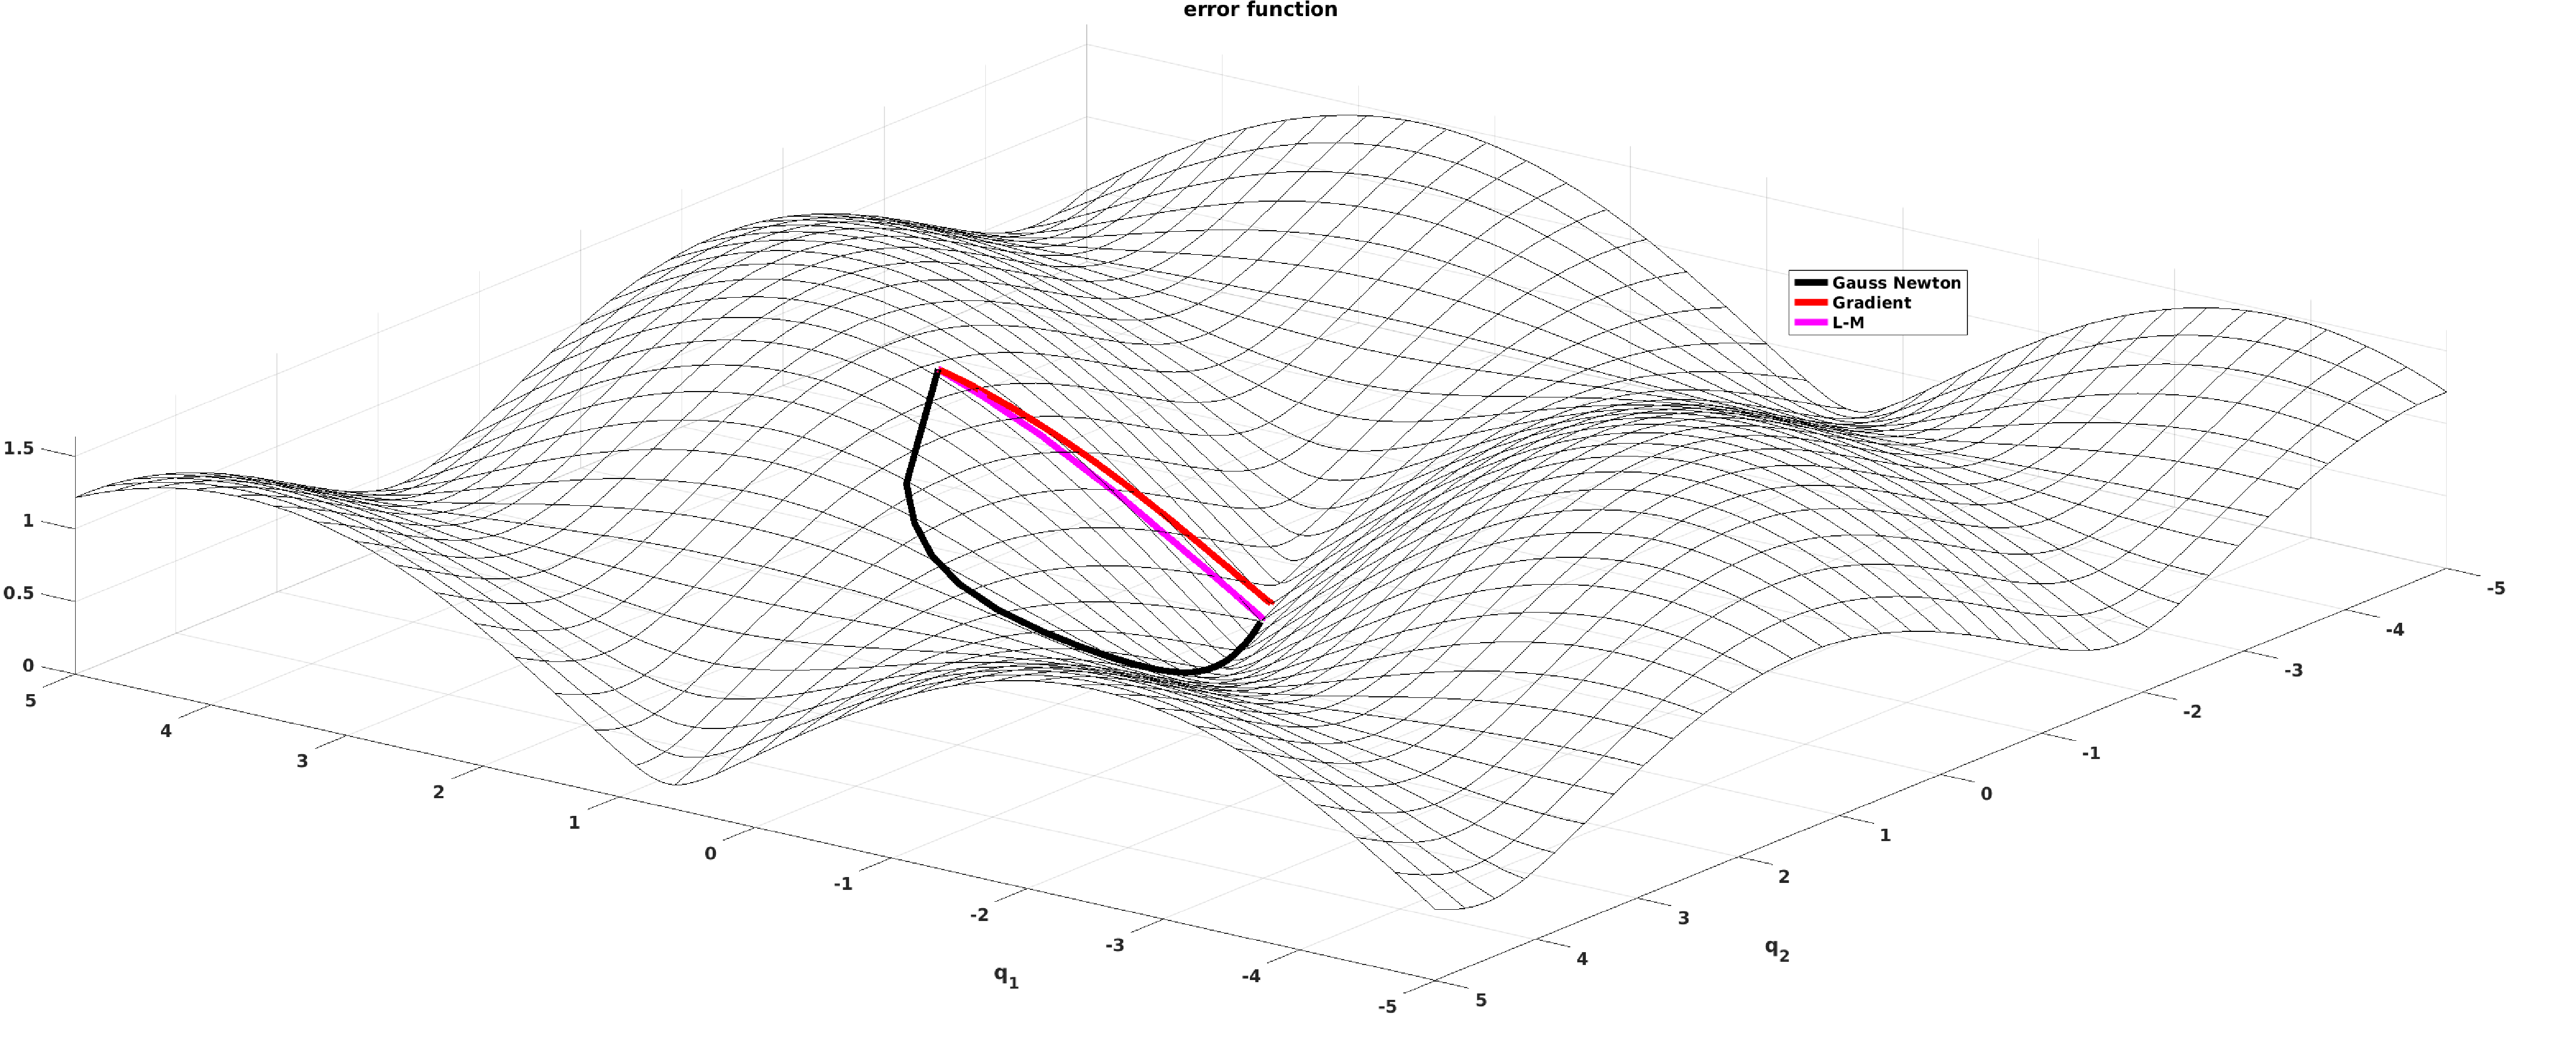
\includegraphics[scale=0.14]{plot/kinematic/error_functin.pdf} 
\caption{Comparison among the three inverse kinematic methods} 
\label{fig:comparison_IK_methodsS}
\end{figure}


\begin{table}[H]
\centering
\begin{tabular}{|l|c|c|c|}
\hline
Method          & error [m]       &  iterations [\#] & elapsed time [s]    \\
\hline
Gradient      & 8.486842e-03     & 500   &   50.189070     \\
Newton        & 9.567838e-06     & 117   &   9.881217     \\
L-M           & 9.710972e-05   & 29    & 15.078741       \\
\hline
\end{tabular}
\caption{comparison among Gradient methood, Newton method and Levenberg-Marquardt method}
\label{tab:comparison}
\end{table}

\section{Space to Time conversion}

The values that I found through the inverse kinematics cannot be passed directly to the robot, since these values are function of the hip displacement, then it is necessary to perform a  conversion during the robot motion. The idea to perform this conversion is to define a constant control cycle  $T$ and compute the conversion of the joints angles; however this is not a trivial problem, because $T$ is different from the SQD time step $\Delta t$ that is also variable, depending on the robot speed. The problem that we have to address is that if $T<\Delta t$ then one SQD step passes in many control cycles, on the other hand if $T>\Delta t$ then many SQD steps pass in one control cycle. In order to compute the joint values at the current control cycle, it is necessary to compute the next time node $t_{k+1}$ using $\Delta t$ given by (\ref{eq:sampletime})using the actual robot speed. If $t_{k+1}>t_{now}$, where $t_{now}$ is the current time incremented at every control cycle of $T$, then it is possible to compute the joint values making an interpolation between two adjacent SWP node. Otherwise increase the node index $k$ and it is necessary to compute again the time until it is larger than $t_{now}$.

\newpage

\section{Simulation and Results}

The simulations that I performed was done using Matlab, on a Linux Ubuntu 20.04.2 LTS with Intel Core™ i7-8550U CPU @ 1.80GHz × 8 . The first problem that I addressed is to solve the optimization problem given by the cost function (\ref{eq:cost_function}) and constraints (\ref{eq:com_evolution}), (\ref{eq:SQD}) and (\ref{eq:vel_const}). 
In order to define the optimization problem in Matlab I used Yalmip, that is an external library of Matlab that allows us to define the cost function, the constraints and to call the solver. This latter can be chosen among all the available solvers, otherwise if one does not specify any solver it chooses the suitable one. In my case I used the solver "\verb+fmincon+", because it is available on Matlab for free; it is not the best solver, as a matter of fact the computation time to find the optimal solution is quite long.\\
I solved this problem for two different values of $\beta$: $\beta = 1.5$ and 
$\beta = 50$. In case of $\beta = 1.5$ it is possible to see from the figure (\ref{fig:opt_x_150_space} that the ZMP trajectory obtained does not track the reference well, but if we look at the velocity profile in figure (\ref{fig:opt_vx_150_space}), it follows the desired profile as much as possible except for the unavoidable oscillations. On the other hand, if we use 
$\beta = 50$, we can see in figure (\ref{fig:opt_x_50_space}) that the obtained ZMP  tracks well the reference  but the velocity profile it is worse with respect to the previous case as it is possible to see from figure (\ref{fig:opt_vx_50_space}).
Under the above discussion, I plot the simulation of three steps having chosen $\beta=50$  both in space discretization and time discretization  (\ref{fig:steps_NOsqd}).

Although in a real robot the ZMP coincides with the ZMP measured from the force/torque sensors at the foot and never exists outside the support polygon \cite{HumanBook}, when calculating the ZMP from the simulated motion of the robot, usually it is used a "precondition" such that the sole keeps the surface contact with the ground since it is fixed to the ground. Instead in my case I do not use this precondition and then it could happen that the ZMP goes outside the SP, as it is shown in figure \ref{fig:opt_x_150_NO_SQD}. To overcome this problem it is necessary to tune properly the weight in the cost function of the optimization problem, such that the ZMP always lies in the SP.

\begin{comment}
%Parte sullo zmp che esce dal support polygon
Although in a real robot the ZMP coincides with the ZMP measured from the force/torque sensors at the foot and never exists outside the support polygon \cite{HumanBook}, when calculating the ZMP from the simulated motion of the robot, we usually use a "precondition" such that the sole keeps the surface contact with the ground since it is fixed to the ground. As a matter of fact, in our simulation, the ZMP is slightly outside the SP as we can see in figure (\ref{fig:opt_x_150_NO_SQD})\\
%
\end{comment}
Converting the result from space to time (\ref{eq:st_conversion}) it is also possible to visualize the same results expressed in function of time in figures (\ref{fig:opt_x_150_time}),(\ref{fig:opt_vx_150_time}),(\ref{fig:opt_x_50_time}) and (\ref{fig:opt_vx_50_time}).

For what concerns the lateral motion, it is not possible to solve the problem with SQD since the motion along the y axis is oscillatory so  the velocity is bounded between a certain positive value  and a negative value, so it passes trough $v_i=0$ and that is a singularity for the model. As a consequence I solved the optimization problem directly in the time domain that is also simpler to solve, since I have a linear convex problem, and it does not affect the flexibility of the SQD along the longitudinal axis. The result of the motion along the coronal axis are reported in figure \ref{fig:opt_y_150_space} for the case with $\beta = 1.5$ and in figure \ref{fig:opt_y_50_space} for the case with $\beta = 50$
After these simulations, I analyzed the same problem but directly in the time domain, with a fixed time discretization, we can see the results from figure (\ref{fig:opt_x_150_NO_SQD}) to figure (\ref{fig:steps_NOsqd}). Comparing these two techniques, we notice that we have similar results. The main difference is that using the SQD we have a  quite high computation time, i.e about 11 hours, versus few seconds in the time discretization case; probably this time could have decreased by using a powerful solver.

Once solved the previous optimization problem I considered the kinematics of the robot by computing the joint values at each discretization step, after that I visualized the result on a biped walker that I developed in Matlab. In particular I developed two different kind of biped walker, the first one has two legs with 3 DoF on each leg, as shown in figure \ref{fig:biped_walking3dof}, instead the second one has two leg with 5 DoF on each leg, as shown in figure \ref{fig:biped_walking12dof}. In order to compute the inverse kinematics I considered the CoM trajectory along x and y resulting from the optimization problem, and also I defined the trajectory of the CoM along z using a composition of two kind of functions, a parabola and a constant function, as it is possible to see from the following equation.


\begin{equation}
  f(x) = \begin{cases} -0.3750x^2+0.81\qquad \qquad \quad \quad \quad if  \> x \in [0,0.2) \\
   0.7951 \qquad \qquad \qquad \qquad   \qquad \quad \quad if x \in [0.2,0.3) \\
   -0.3750x^2+0.375x+0.7162 \quad \quad if  \> x \in [0.3,0.7) \\
   0.7951 \qquad \qquad \qquad \qquad   \qquad \quad \quad  if x \in [0.7,0.8) \\
    -0.3750x^2+0.75x+0.4350\quad \quad \quad if  \> x \in [0.8,1.2) \\
   0.7951 \qquad \qquad \qquad \qquad   \qquad \quad \quad  if x \in [1.2,1.5)\end{cases} \\
\end{equation}

In order to solve the inverse kinematics problem I design a trajectory for the heel. Since this trajectory has a particular shape, figure \ref{fig:foot_trajectory}, it is not very easy to define it by functions, then I have designed this trajectory by hand using the Matlab toolbox called \textit{singEditor}, after that I extracted the data and saved as an array of samples in the work-space of Matlab. 
At the end I used this data as a reference trajectory of the heel for one footstep, taking care to adjust it during the inverse kinematics computation. In fact, since this trajectory has been designed by hand, it could happen that in a certain point the distance from the CoM and the heel is larger than the length of the leg, so I force the leg to pass through a singularity and as I said in section \ref{sec:KWP} this is a problem for the Newton method. To overcome this problem at each discretization step I check the distance between the CoM and the heel and if this distance is larger then the length of leg I increase the values of the heel along the $z$ axis, so that this distance reaches, at most, the value of the length of the leg.  In analogy of a generic manipulator the CoM trajectory along x,y and z represent the base frame position, instead the trajectory of the heel is the end effector position. Using this two trajectories, i.e. the base trajectory and the end effector trajectory, I computed the inverse kinematics using the Newton method for the two kinds of biped walkers. But first I defined the forward kinematic by assigning the reference frame of each joint  for the 3 DoF model as shown in fig \ref{fig:3dof_frame} and for the 5 DoF model as shown in fig \ref{fig:5dof_frame}, and then I computed the DH tables respectively  tab \ref{tab:DH_3dof} and \ref{tab:DH_5dof}.


\begin{figure}
\centering
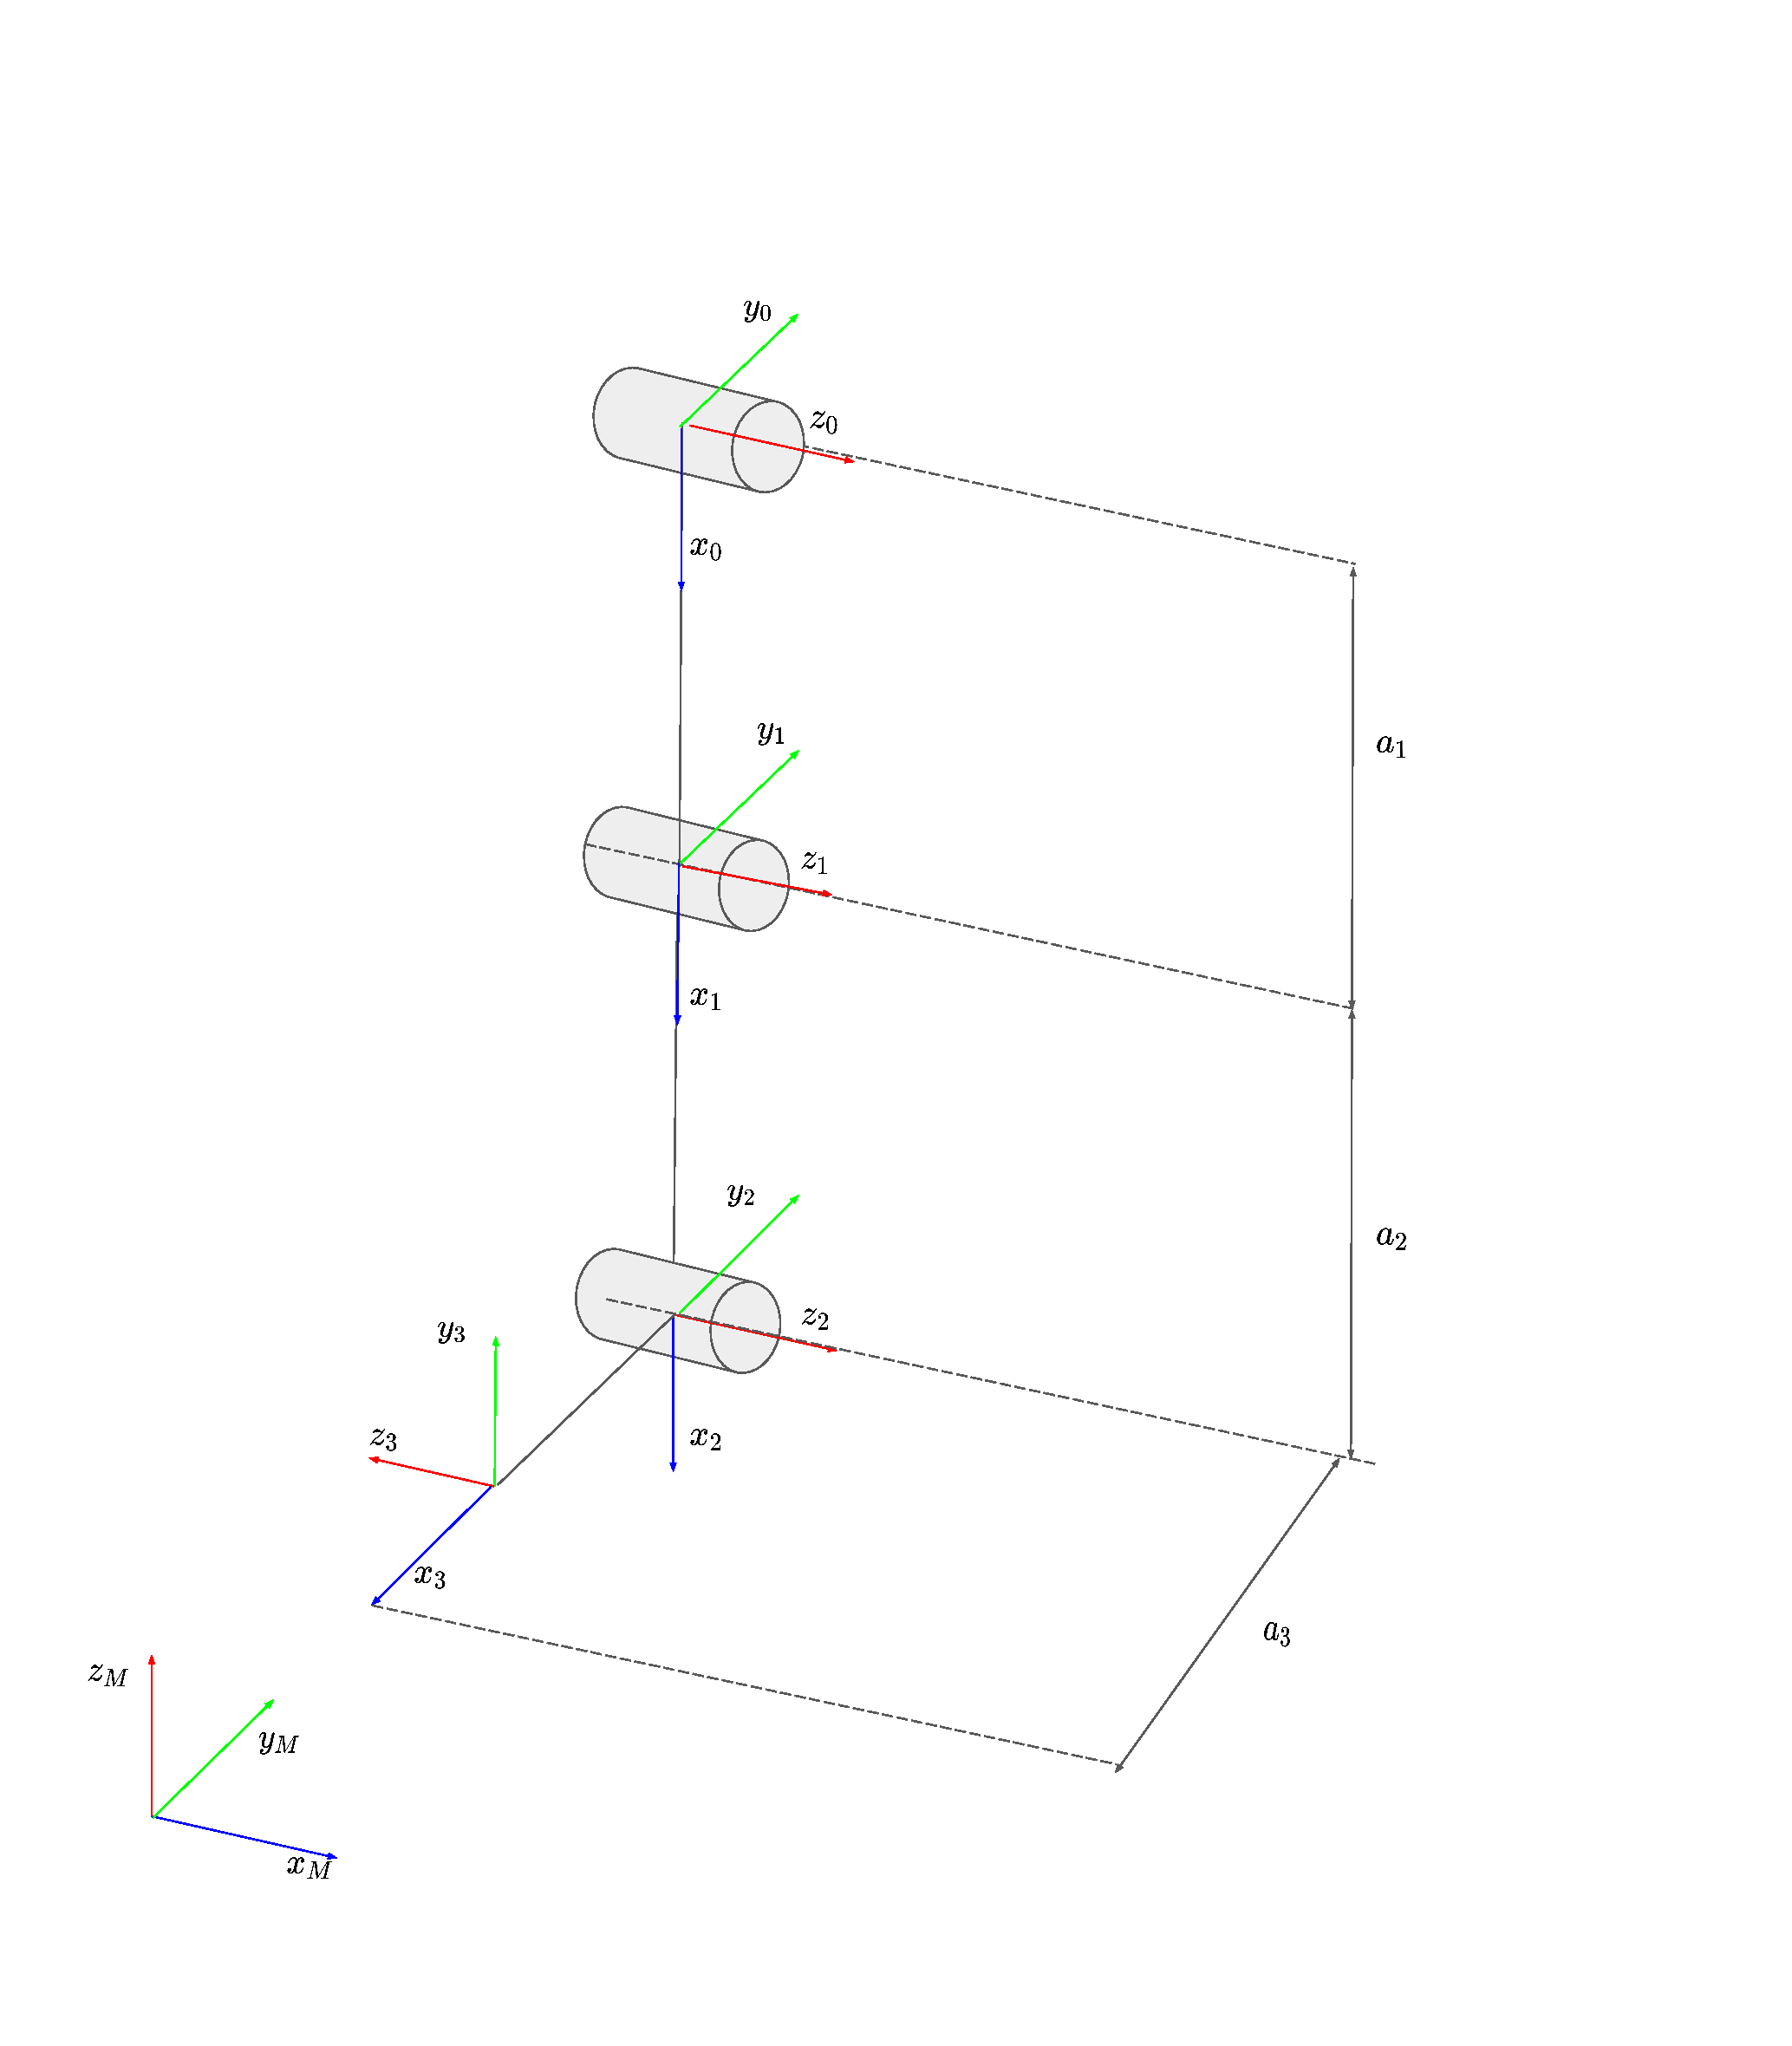
\includegraphics[scale=0.4]{plot/kinematic/3dof_leg.pdf} 
\caption{Frame assignment to the 3 DoF leg} 
\label{fig:3dof_frame}
\end{figure}

\begin{figure}
\centering
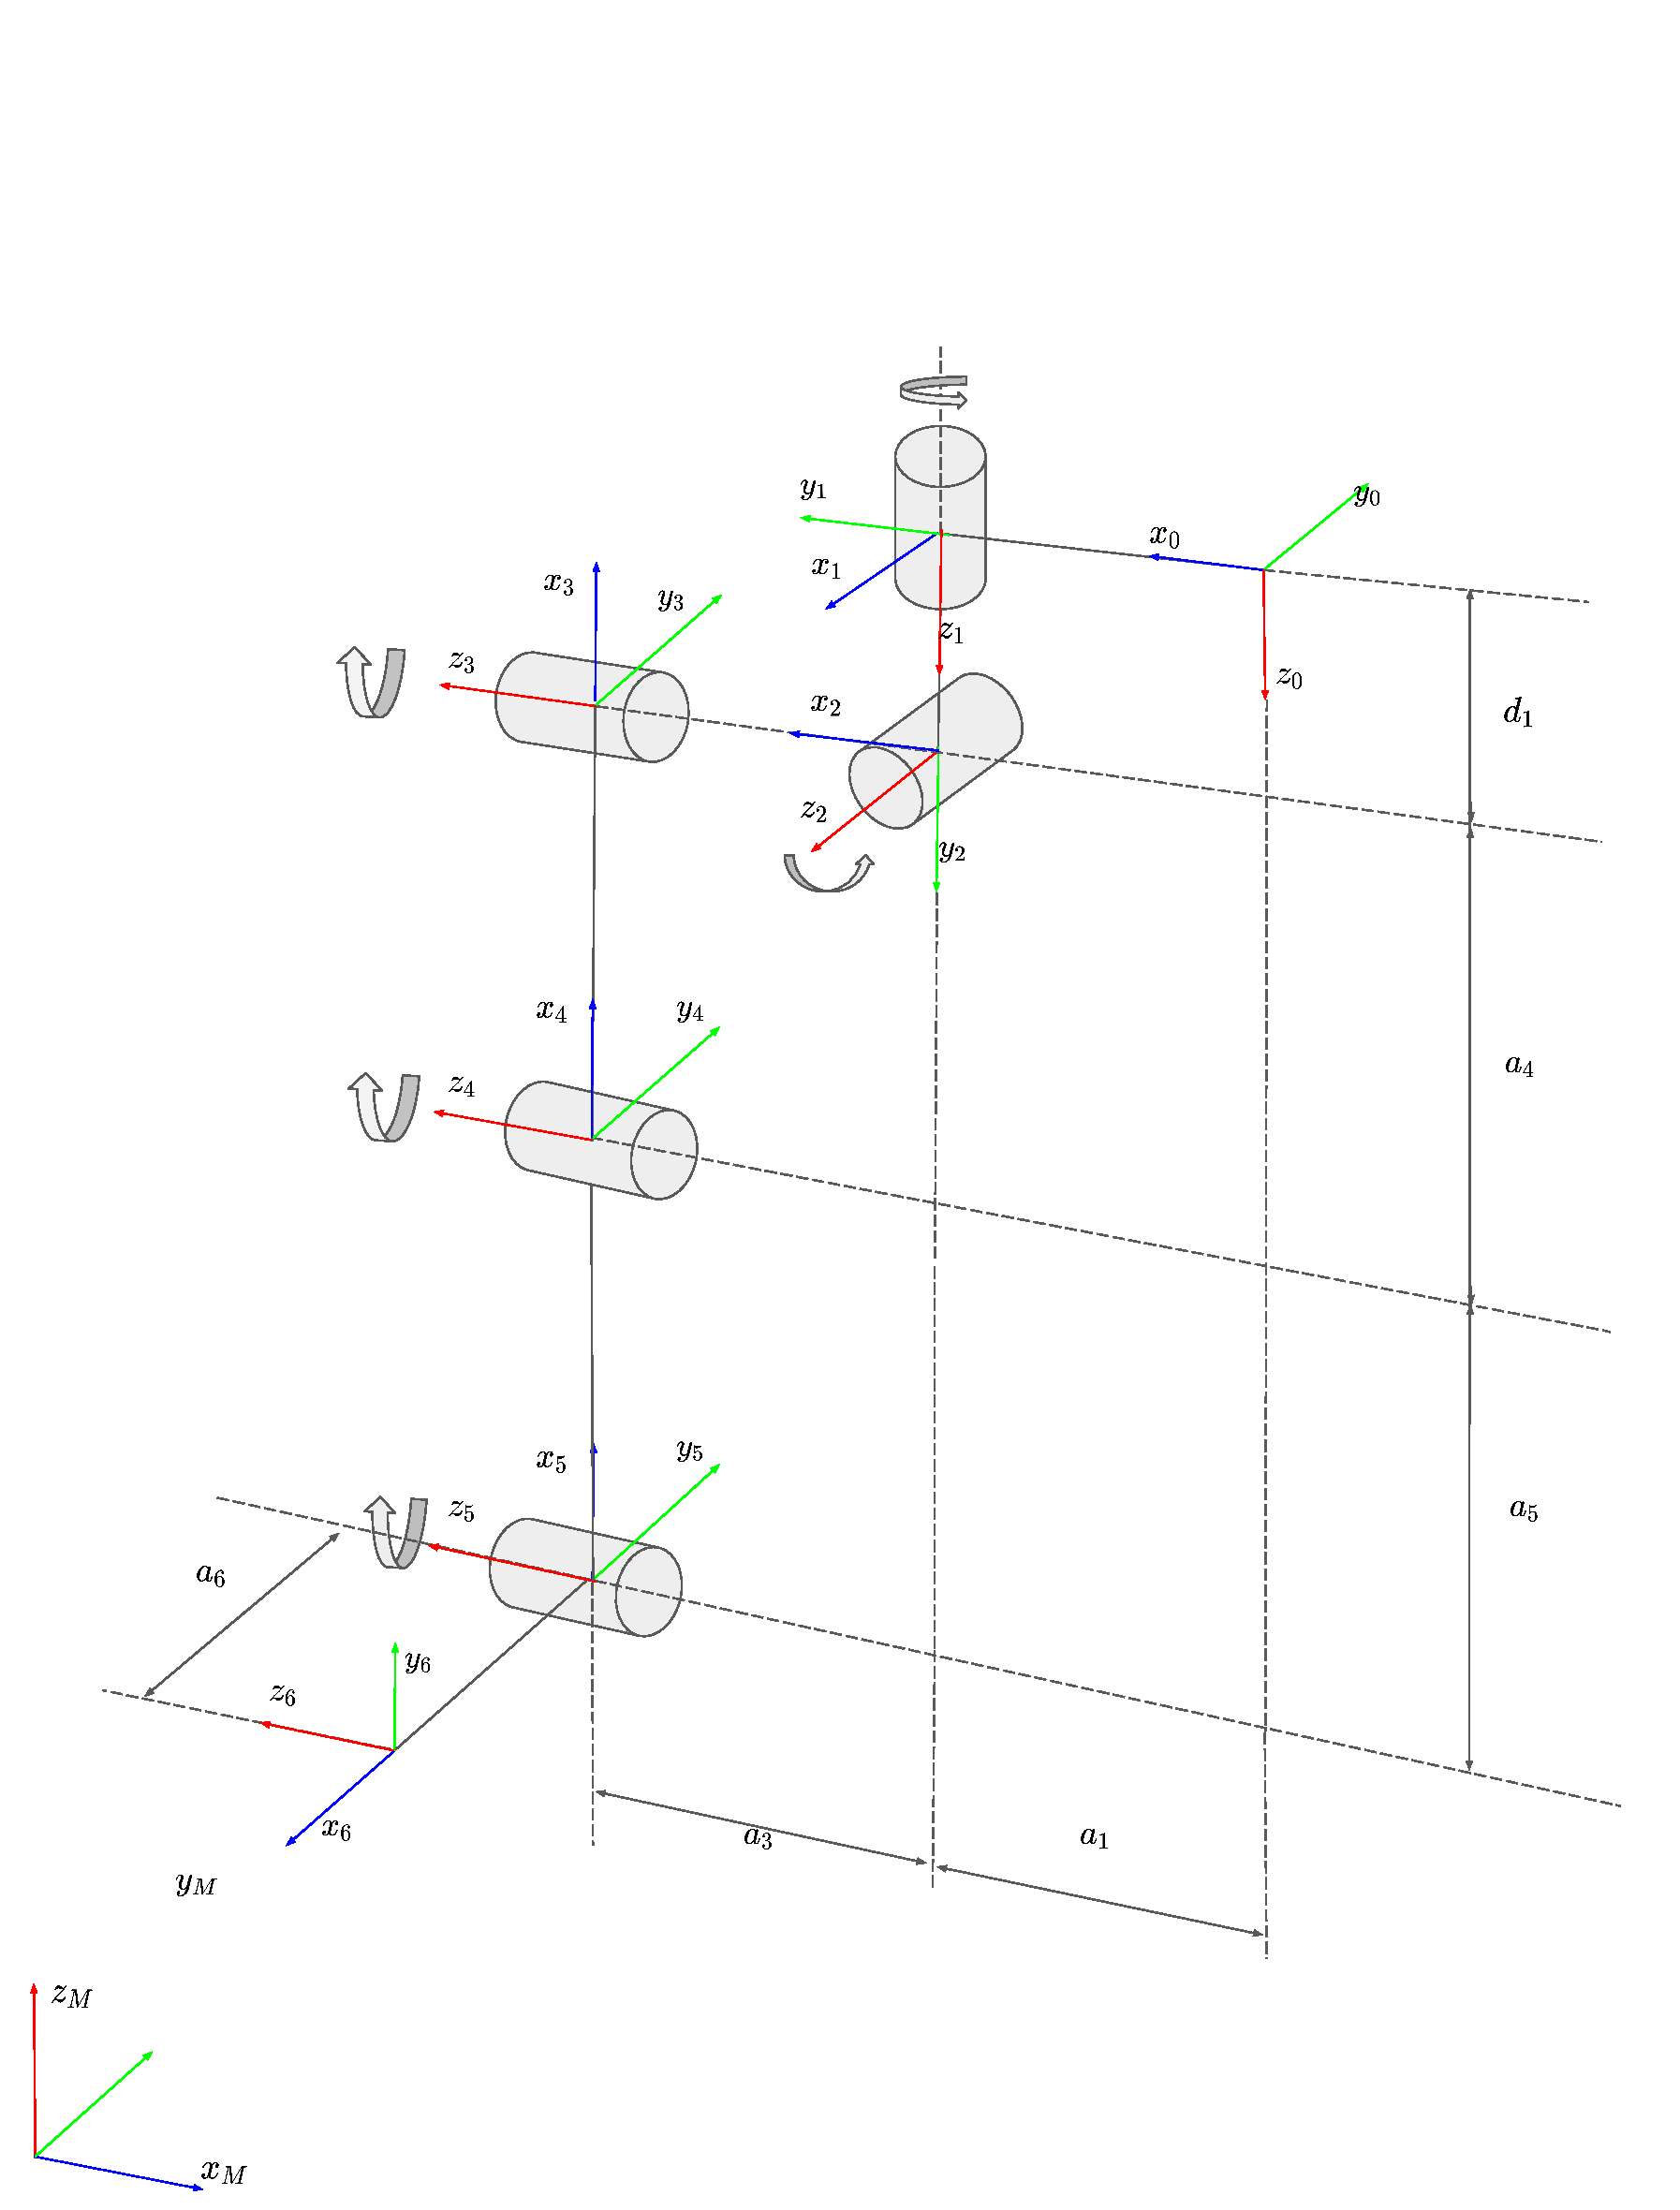
\includegraphics[scale=0.4]{plot/kinematic/5dof_leg.pdf} 
\caption{Frame assignment to the 5 DoF leg} 
\label{fig:5dof_frame}
\end{figure}


\begin{table}
\begin{minipage}[b]{0.48\textwidth}
\centering
\begin{tabular}{|c|c|c|c|c|}
\hline
$i$          & $\alpha_i$        &  $a_i$ & $d_i$ & $\theta_i$    \\
\hline
1      & 0     & 0.41   &   0 &   $\theta_1^{\star}$ \\
\hline
2        & 0     & 0.41   &   0   & $\theta_2^{\star}$ \\
\hline
3          & 0   & 0.15    & 0      & $\theta_3^{\star}$\\
\hline
\end{tabular}
\caption{DH table 3 DoF model}
\label{tab:DH_3dof}
\end{minipage}
\begin{minipage}[b]{0.48\textwidth}
\centering
\begin{tabular}{|c|c|c|c|c|}
\hline
$i$          & $\alpha_i$        &  $a_i$ & $d_i$ & $\theta_i$    \\
\hline
1      & 0     & 0.025   &   0.2 &   $\theta_1^{\star}$ \\
\hline
2        & $\pi/2$     & 0   &   0   & $\theta_2^{\star}$ \\
\hline
3          & $-pi/2$   & 0.075    & 0      & $\theta_3^{\star}$\\
\hline
4      & 0     & 0.41   &   -0.39 &   $\theta_4^{\star}$ \\
\hline
5        & 0     & 0.41   &   -0.41   & $\theta_5^{\star}$ \\
\hline
6          & 0   & 0.15    & -0.15      & $\theta_6^{\star}$\\
\hline
\end{tabular}
\caption{DH table 5 DoF model}
\label{tab:DH_5dof}
\end{minipage}
\end{table}

I collected all the values computed with the inverse kinematics, of one leg, in an array of vectors  where the dimension of the array is equal to the number of the SQD steps, then using  the values of one leg I computed the values of the other leg by translating the vectors in the array, figure \ref{fig:left_leg_joints} and \ref{fig:right_leg_joints} show the evolution in space of the joints respectively of the left leg and the right leg, where the point in which the knee angle crosses the zero value is a singular configuration. 


\begin{figure}
     
        \center
        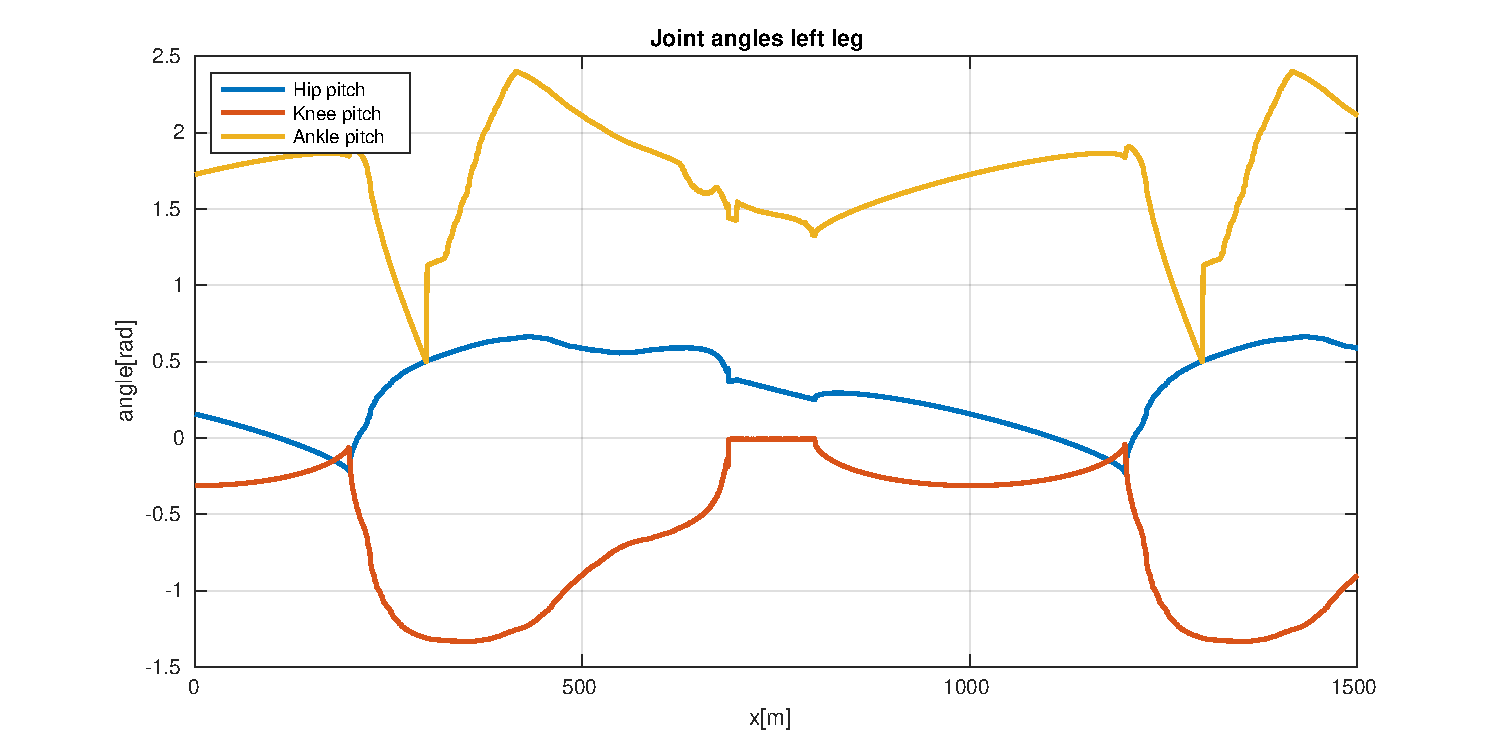
\includegraphics[scale=0.5]{plot/kinematic/left_leg_joints.pdf} 
        \caption{Left leg joint values} 
        \label{fig:left_leg_joints}
  
\end{figure}

\begin{figure}
\center
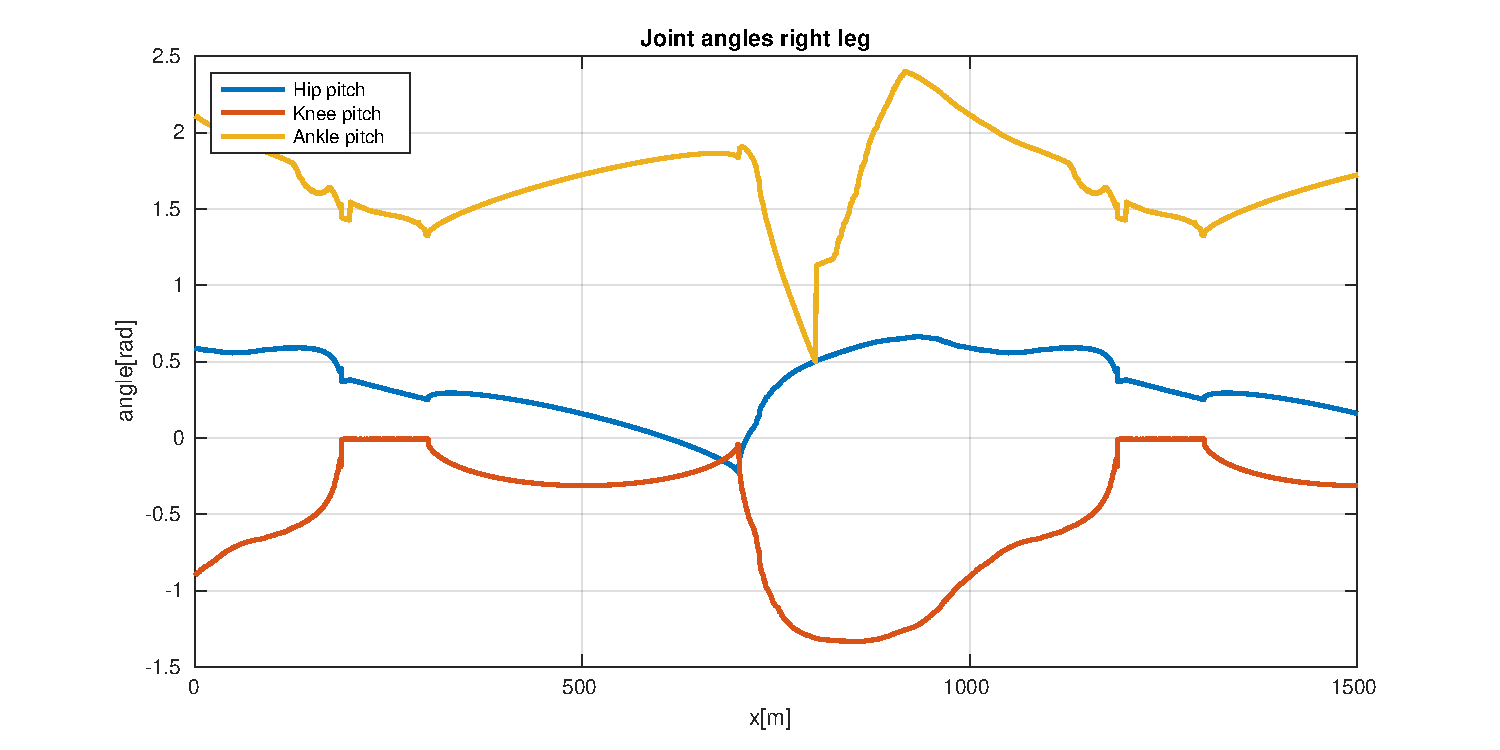
\includegraphics[scale=0.5]{plot/kinematic/right_leg_joints.pdf} 
\caption{Right leg joint values} 
\label{fig:right_leg_joints}
\end{figure}

Additionally I have measured some performance indexes to evaluate the inverse kinematics computation, that I reported in table \ref{tab:KPI_3dof} for the 3 DoF model and in the table \ref{tab:KPI_6dof}  for the 5 DoF model. Clearly the performance of the 3 DoF model are better than the 5 DoF one because the model is simpler, but both have good performance in terms of  convergence in time, number of iterations and Cartesian errors, even if the method used has some problems near singularities.



 \newgeometry{left=0.1cm, right=0.1cm,}

\begin{figure}
\centering
 \begin{minipage}{0.48\textwidth}

    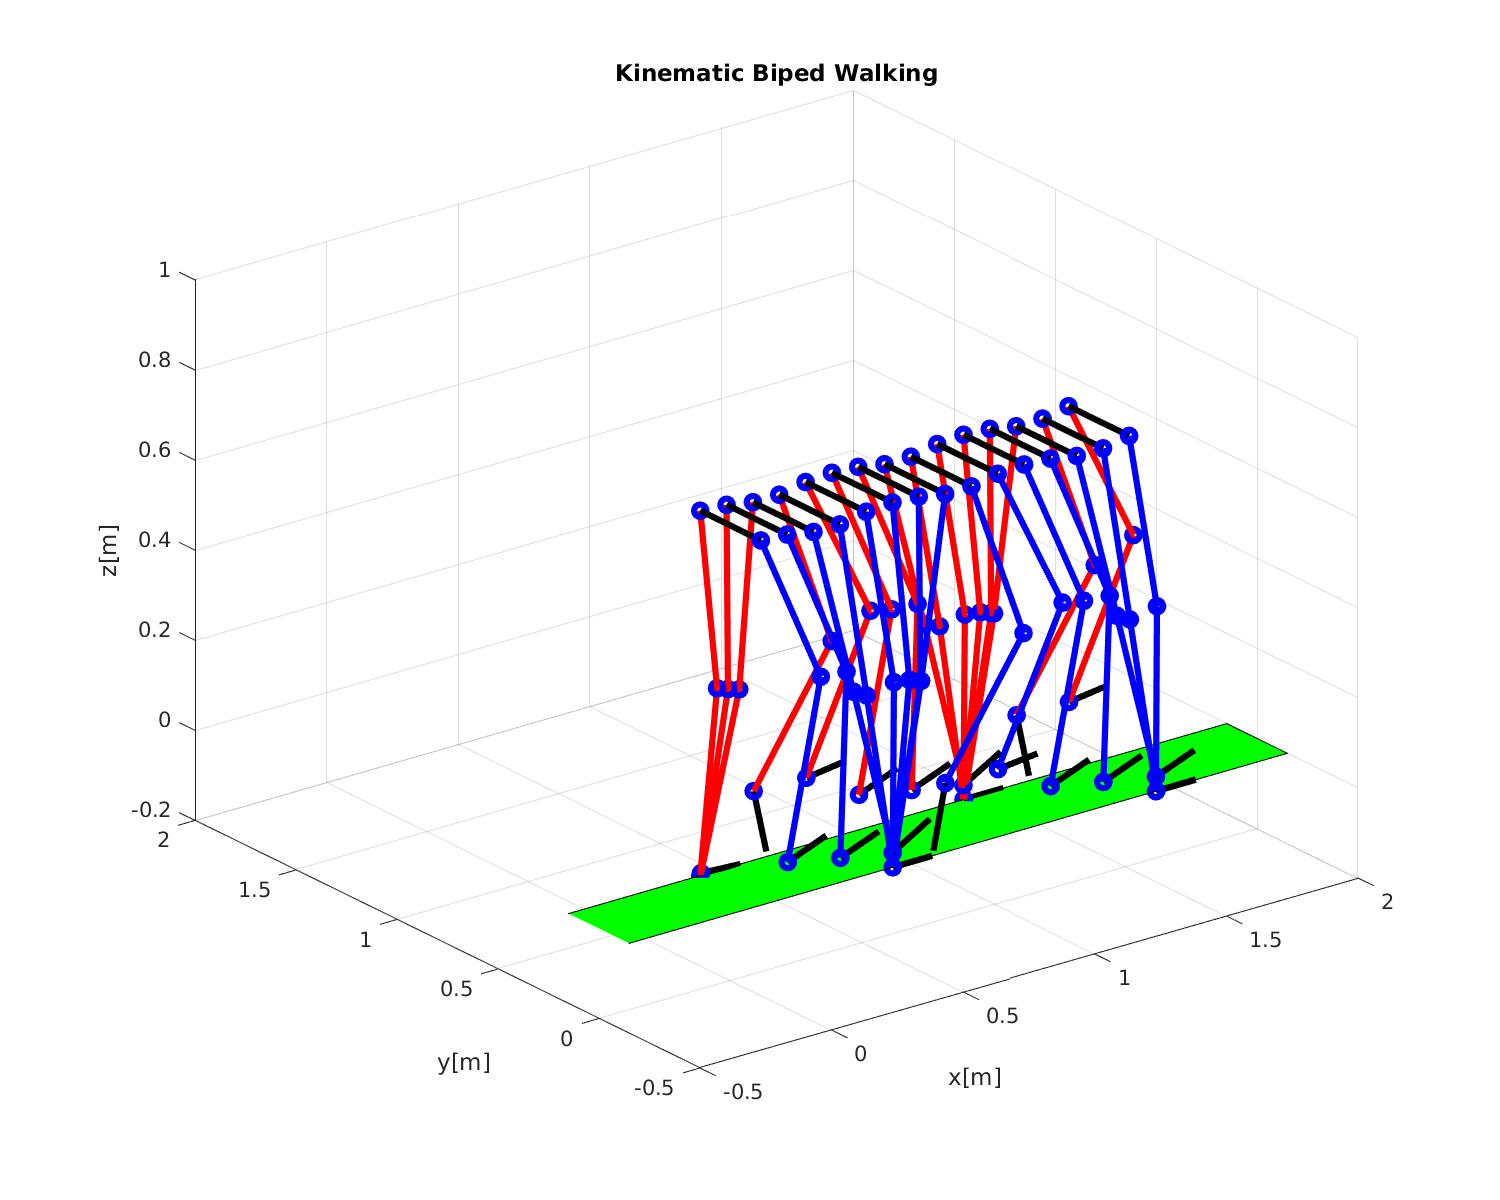
\includegraphics[scale=0.42]{plot/kinematic/biped_walking.pdf} 
    \caption{Some poses of the 5 DoF biped walking} 
    \label{fig:biped_walking3dof}
  \end{minipage}
 
   \begin{minipage}{0.48\textwidth}
     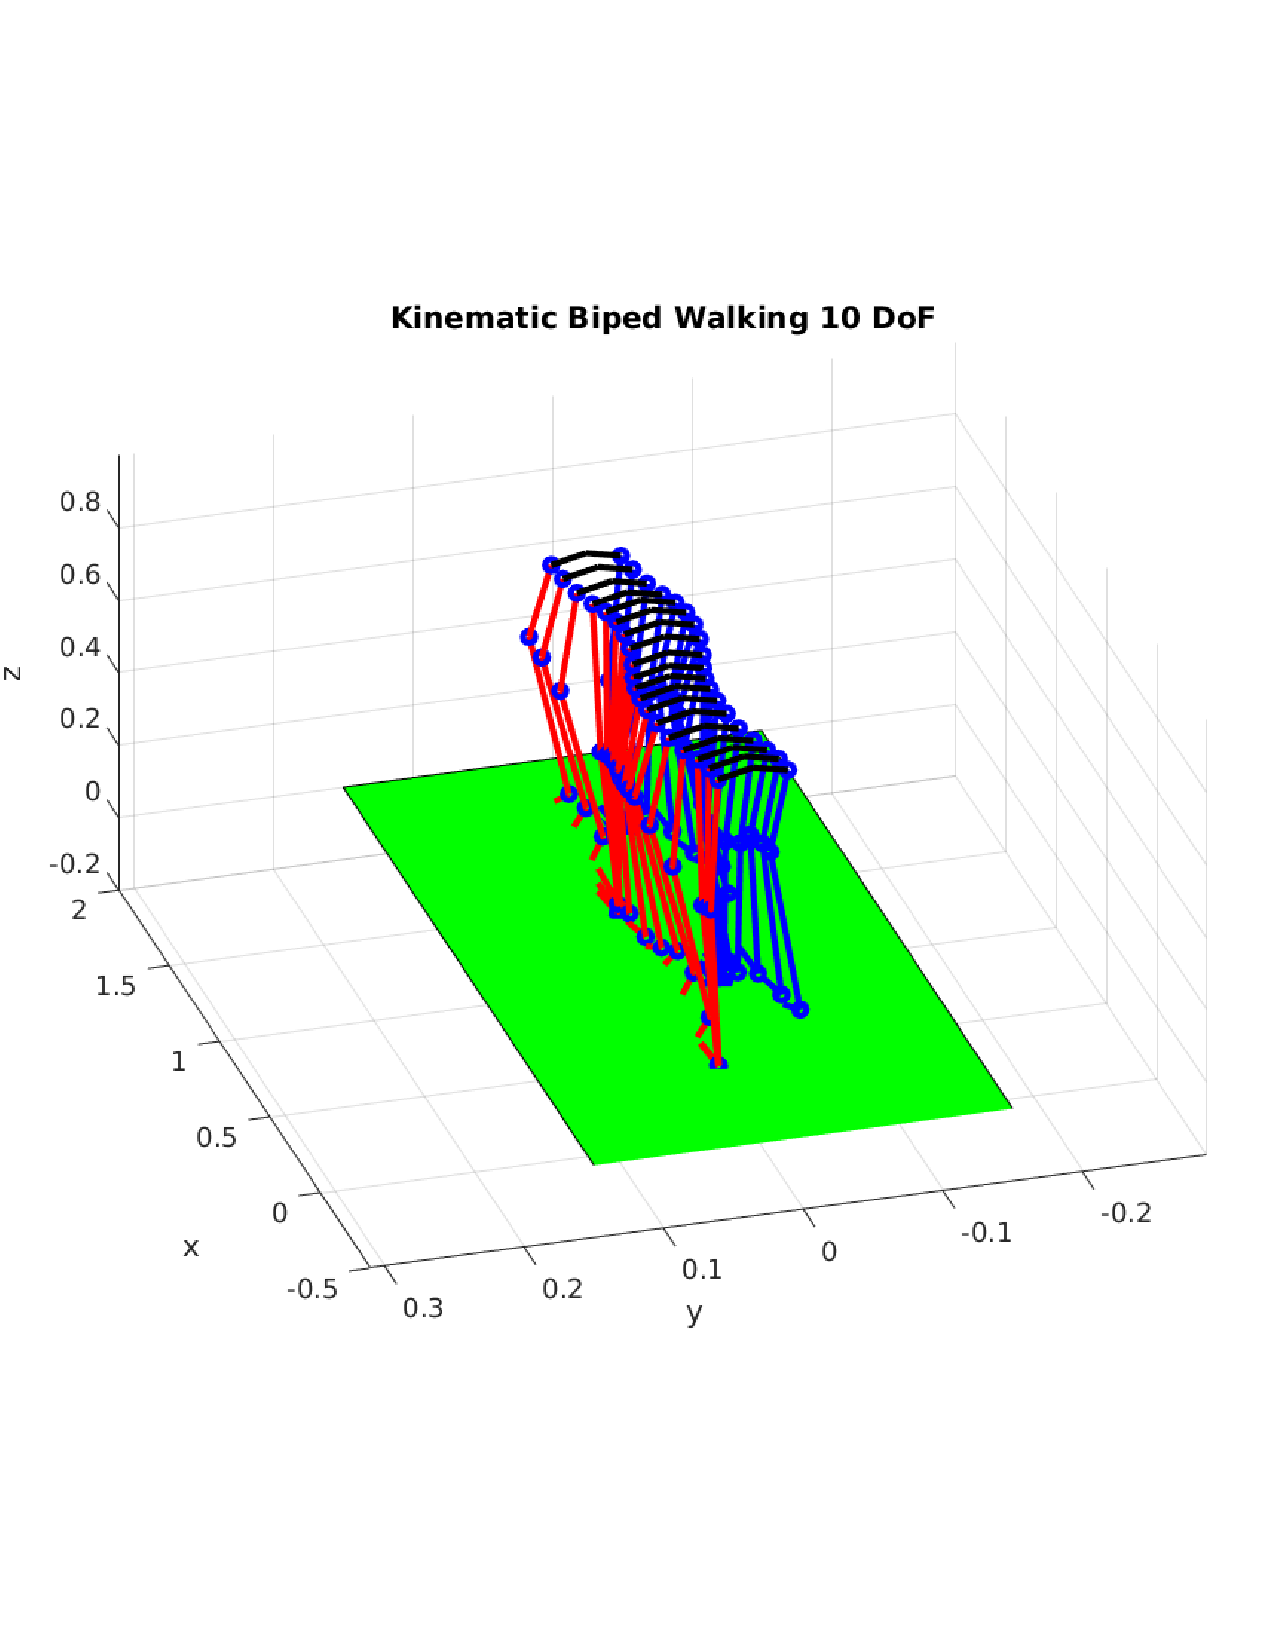
\includegraphics[scale=0.5]{plot/kinematic/biped_walking10dof.pdf} 
        \caption{Some poses of the 10 DoF biped walker} 
        \label{fig:biped_walking12dof}
   \end{minipage}
\end{figure}
\restoregeometry

\begin{table}
\begin{minipage}[b]{0.48\textwidth}
\begin{center}
\begin{tabular}{|l|l|l|}
\hline
\multirow{3}{1.5cm}{Time [ms]}  
&max &  3.053 \\
\cline{2-3} 
&min & 0.011\\
\cline{2-3} 
& avg & 0.065\\
\hline
\multirow{3}{1.5cm}{Iterations [\#]}   
&max & 6\\
\cline{2-3} 
& min & 1\\
\cline{2-3} 
& avg & 1.48\\
\hline
\multirow{3}{1.5cm}{Error [m]} 
&max & 9.982e-07\\
\cline{2-3} 
&min & 1.434e-12\\
\cline{2-3} 
&avg & 1.434e-12\\
\hline
\end{tabular}
\end{center}
\caption{Inverse kinematics performance index for the 3 DoF model}
\label{tab:KPI_3dof}
\end{minipage}
\begin{minipage}[b]{0.48\textwidth}

\begin{center}
\begin{tabular}{|l|l|l|}
\hline
\multirow{3}{1.5cm}{Time [ms]}  
&max &  5.705 \\
\cline{2-3} 
&min & 0.008\\
\cline{2-3} 
& avg & 3.54\\
\hline
\multirow{3}{1.5cm}{Iterations [\#]}   
&max & 31\\
\cline{2-3} 
& min & 1\\
\cline{2-3} 
& avg & 9.29\\
\hline
\multirow{3}{1.5cm}{Error [m]} 
&max & 9.999e-07\\
\cline{2-3} 
&min & 3.852e-08\\
\cline{2-3} 
&avg & 9.198e-07\\
\hline
\end{tabular}
\end{center}
\caption{Inverse kinematics performance index for the 5 DoF model}
\label{tab:KPI_6dof}
\end{minipage}
\end{table}

\begin{figure}
\center
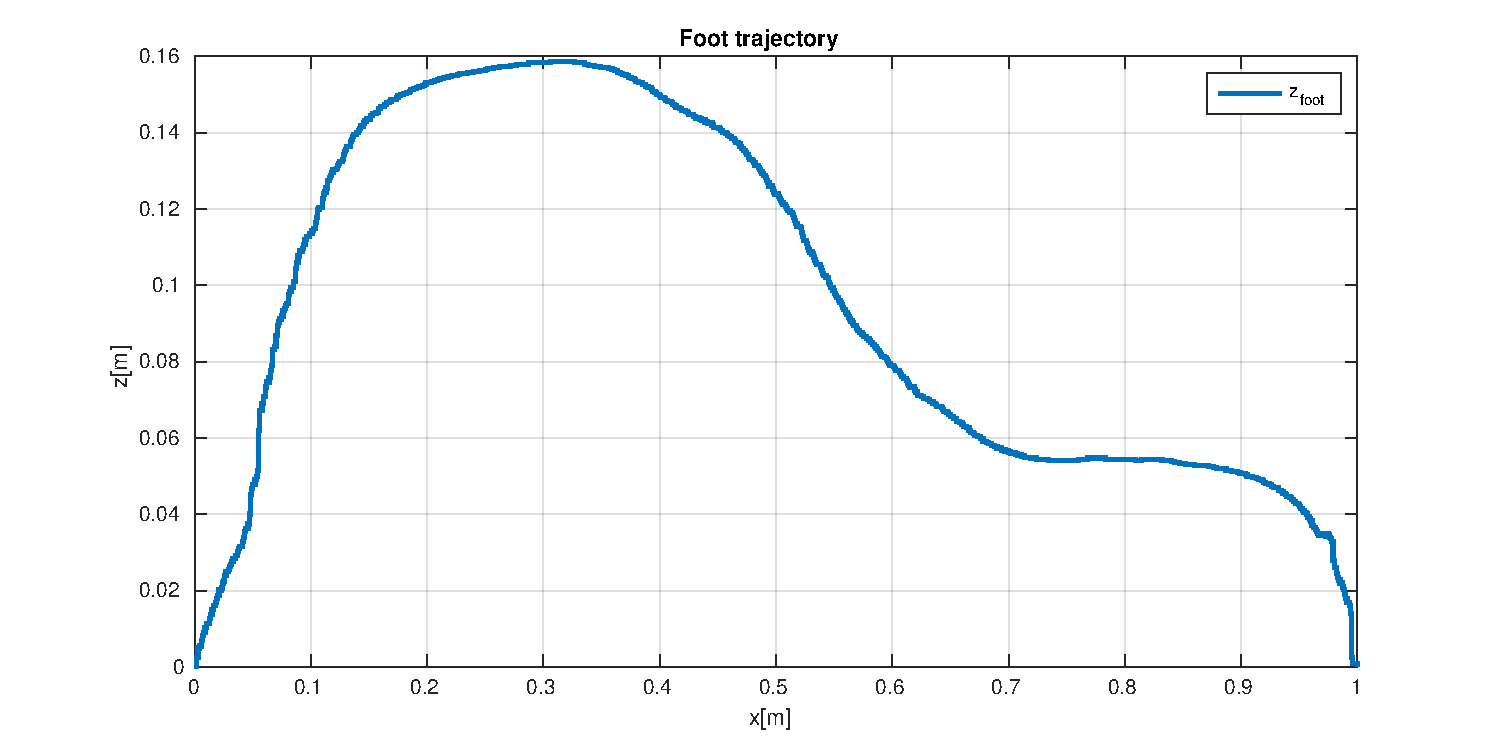
\includegraphics[scale=0.5]{plot/kinematic/foot_trajectory.pdf} 
\caption{Foot trajecotry in function of the hip position} 
\label{fig:foot_trajectory}
\end{figure}


To visualize the two kind of biped walker, I defined a Matlab function that plots a leg , given the base position and its configuration. In particular this Matlab function plots each part of the leg by computing the forward kinematic from the Matlab reference frame to the tip of each  link. After that, in order to plot the two legs I called twice this function inside a loop of $N$ iteration, where $N$ is the number of SQD steps, and at each iteration I passed the configuration found in the inverse kinematic to plot the left leg and the translated one to plot the right leg.



\begin{figure}
\center
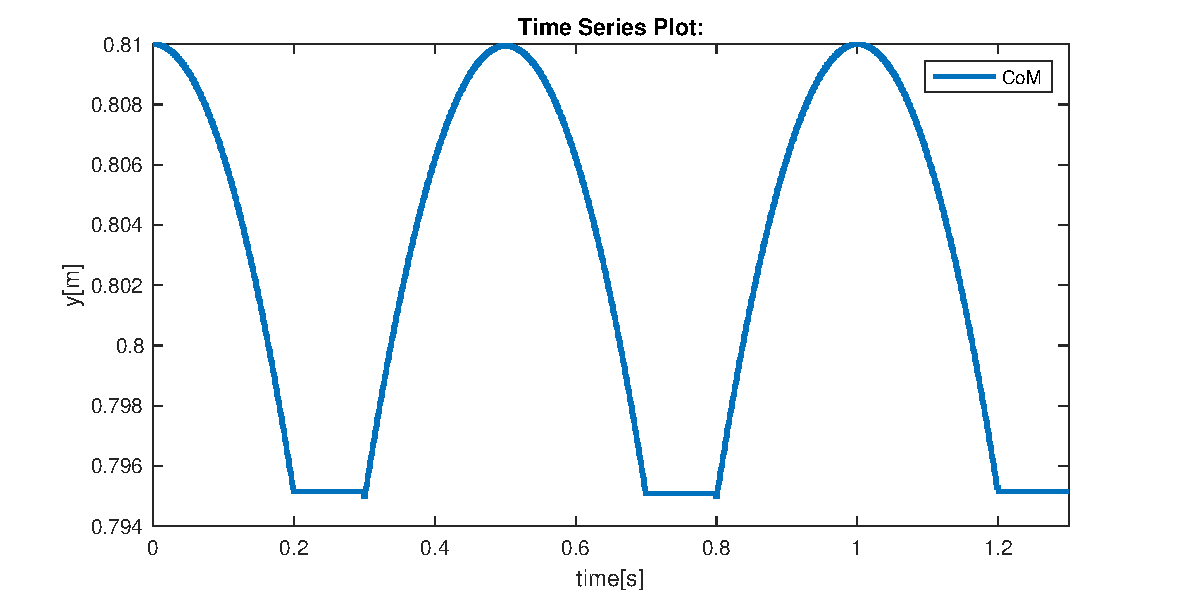
\includegraphics[scale=0.7]{plot/com.pdf} 
\caption{CoM height trajectory } 
\label{fig:COM_HEIGT}
\end{figure}


\begin{figure}
\center
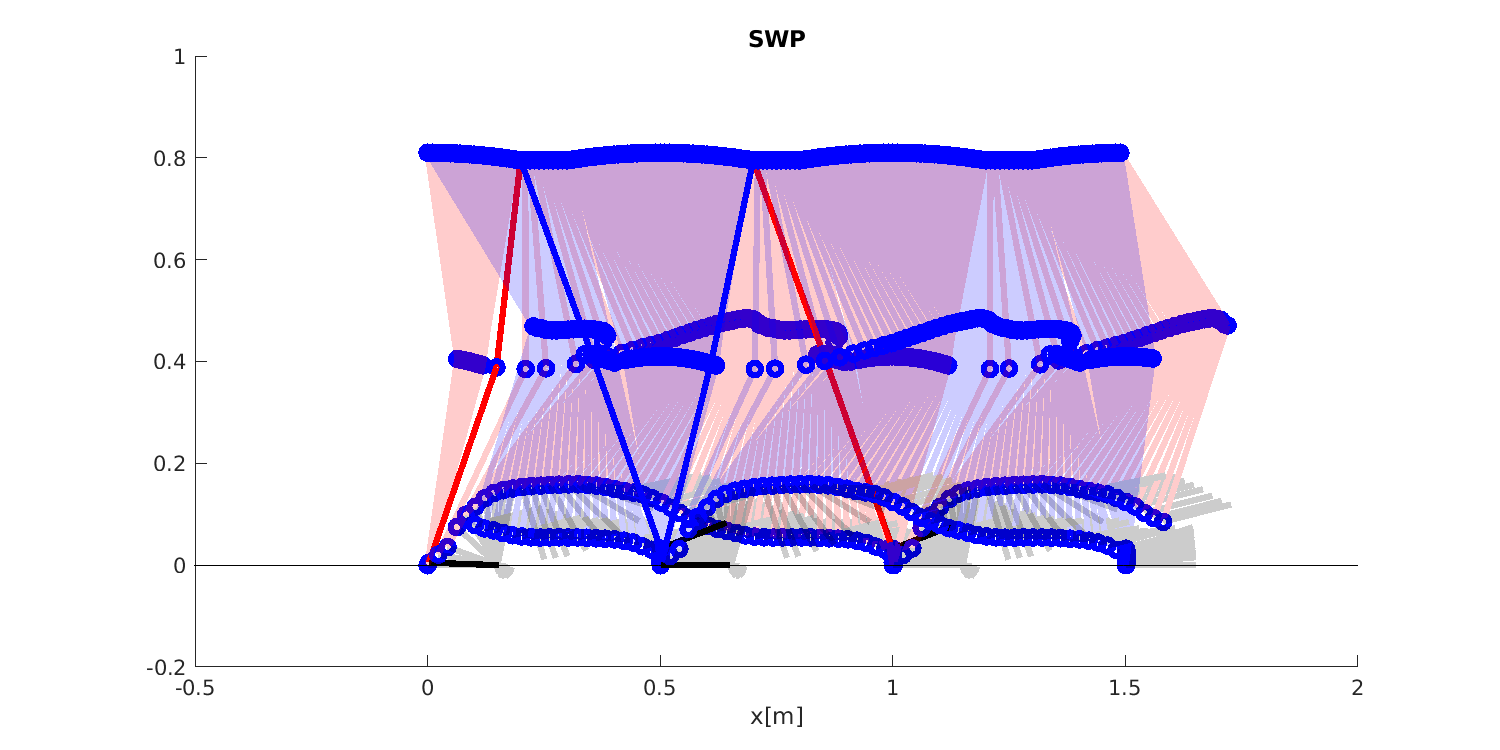
\includegraphics[scale=0.5]{plot/kinematic/SPW.pdf} 
\caption{Spatial Walking Pattern} 
\label{fig:SPW}
\end{figure}


 

 \newpage
% \newgeometry{left=3.3cm, right=3.3cm,}
\begin{figure}
     \begin{minipage}[b]{0.48\textwidth}
       \centering
         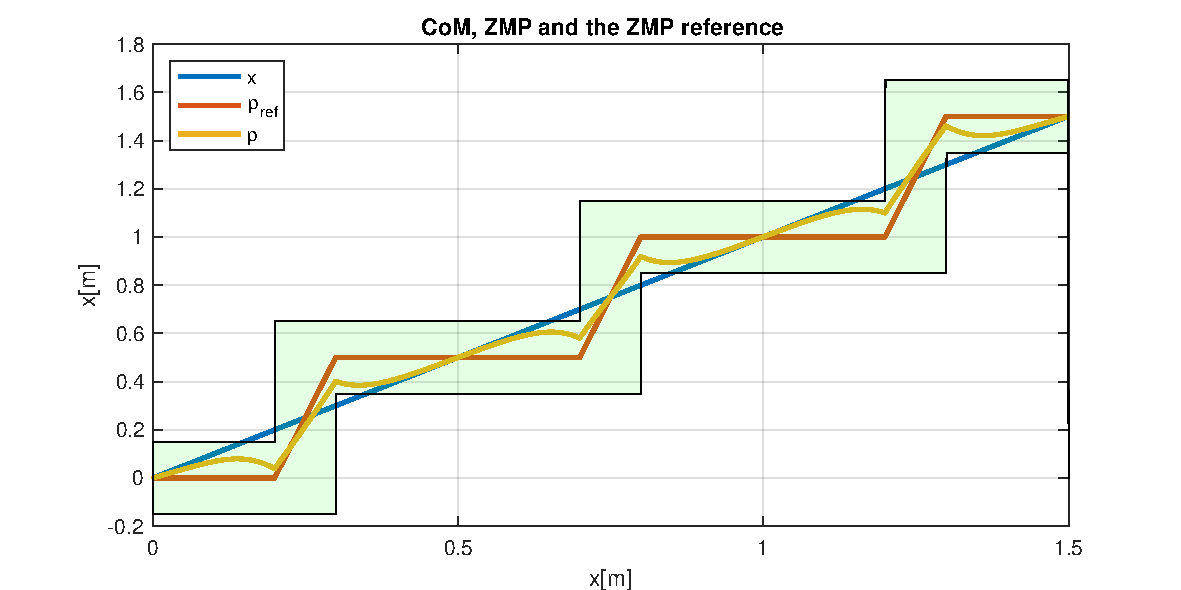
\includegraphics[scale=0.4]{plot/SQD/150/x_opt_150.pdf}
         \caption{ZMP and CoM profile resulting from the optimization with $\beta=1.50$} 
         \label{fig:opt_x_150_space}
     \end{minipage}
    \hfill
     \begin{minipage}[b]{0.48\textwidth}
         \centering
        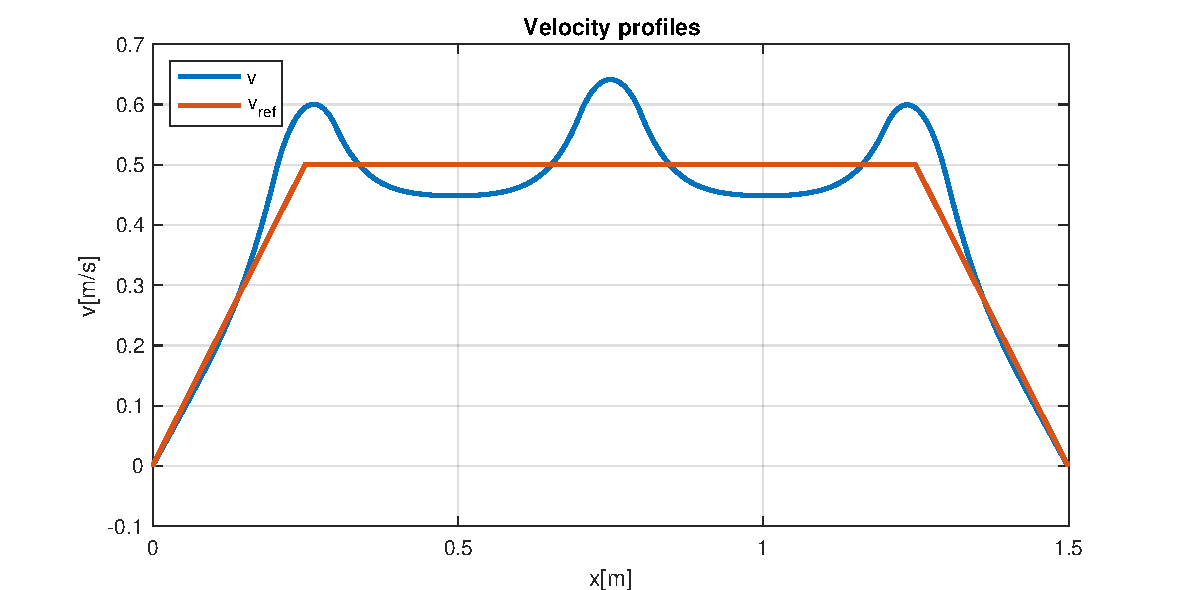
\includegraphics[scale=0.4]{plot/SQD/150/vx_opt_150.pdf} 
        \caption{CoM speed profile resulting from the optimization with  $\beta=1.50$} 
        \label{fig:opt_vx_150_space}
     \end{minipage}   
     \vfill  
     \begin{minipage}[b]{0.48\textwidth}
         \centering
        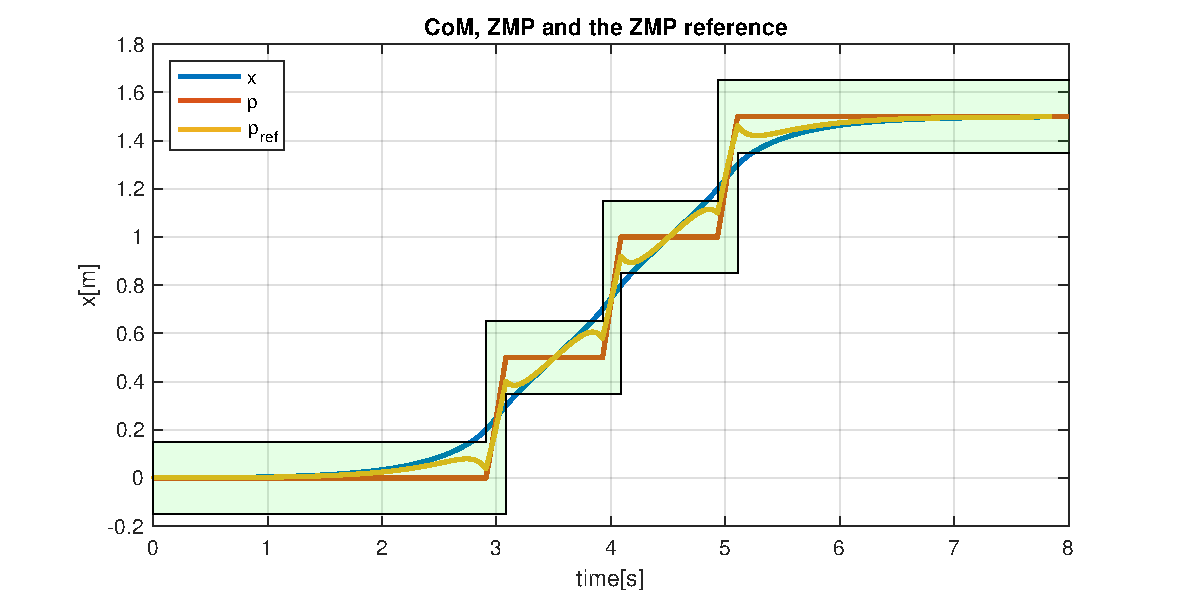
\includegraphics[scale=0.4]{plot/SQD/150/x_time_150.pdf} 
        \caption{ZMP and CoM profile resulting from the optimization in time domain with $\beta=1.50$} 
        \label{fig:opt_x_150_time}
     \end{minipage}  
     \hfill
     \begin{minipage}[b]{0.48\textwidth}
         \centering
        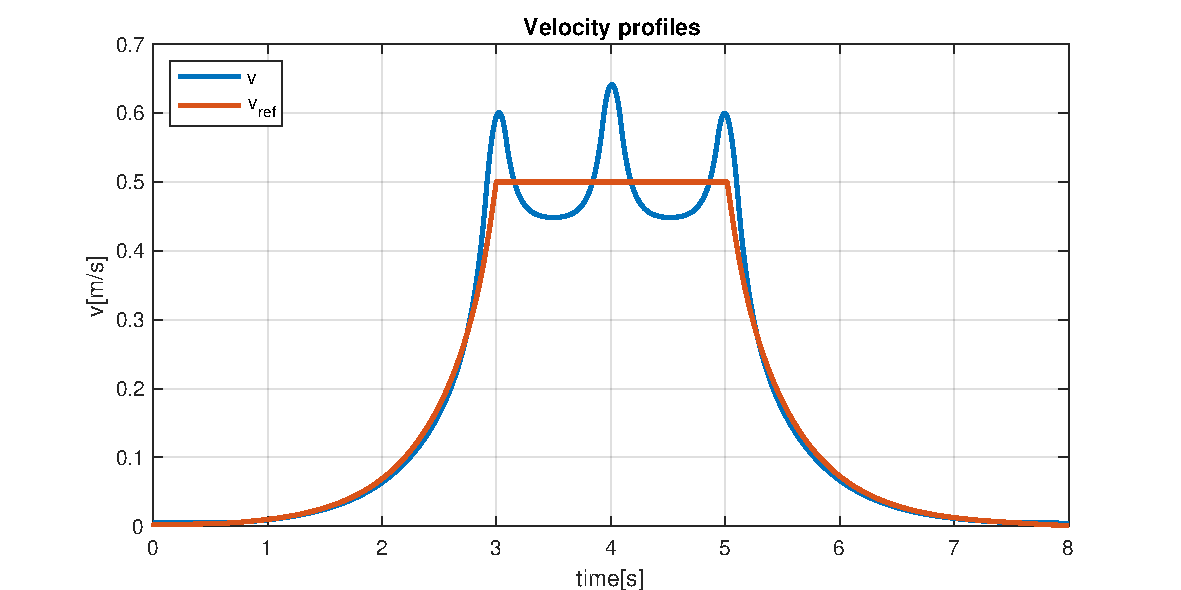
\includegraphics[scale=0.4]{plot/SQD/150/vx_time_150.pdf} 
        \caption{ZMP and CoM profile resulting from the optimization in time domain with $\beta=1.50$} 
        \label{fig:opt_vx_150_time}
     \end{minipage}     
\begin{minipage}[b]{0.48\textwidth}
         \centering
         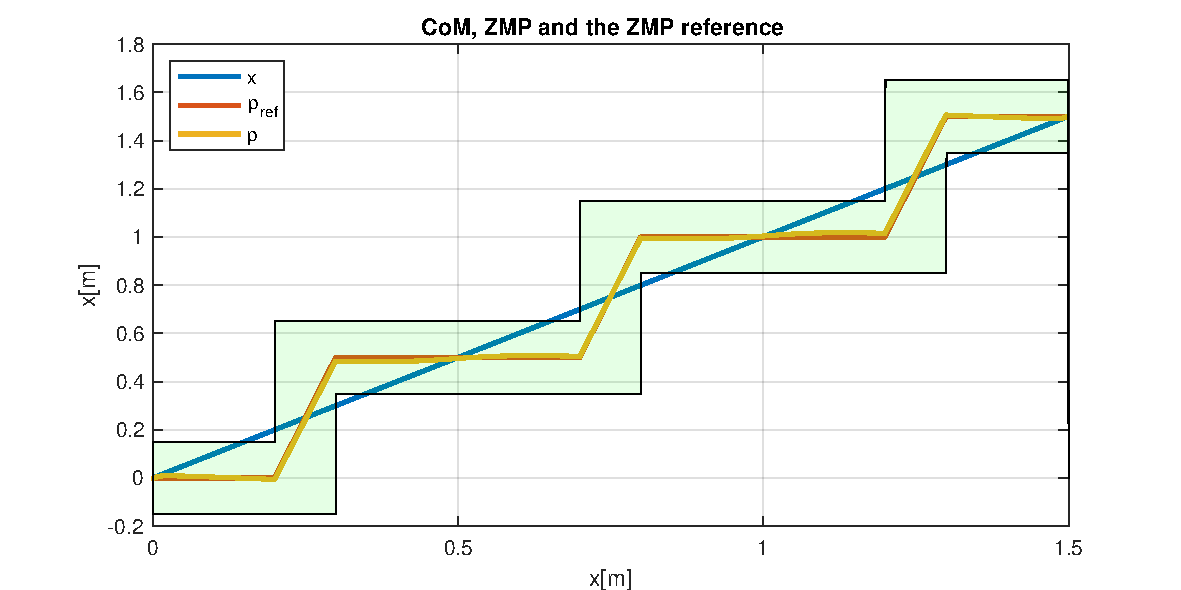
\includegraphics[scale=0.4]{plot/SQD/50/x_opt_50.pdf} 
         \caption{ZMP and CoM profile resulting from the optimization with $\beta=50$} 
         \label{fig:opt_x_50_space}
     \end{minipage}
     \hfill
     \begin{minipage}[b]{0.48\textwidth}
         \centering
        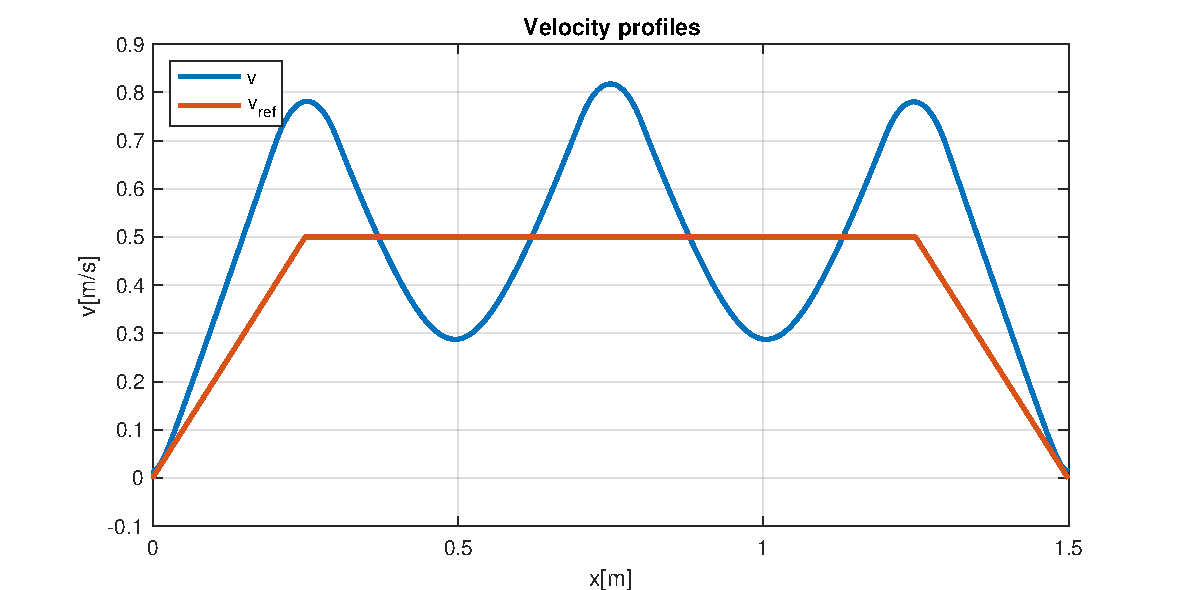
\includegraphics[scale=0.4]{plot/SQD/50/vx_opt_50.pdf} 
        \caption{CoM speed profile resulting from the optimization with $\beta=50$} 
        \label{fig:opt_vx_50_space}
     \end{minipage}   
     \vfill
       \begin{minipage}[b]{0.48\textwidth}
         \centering
        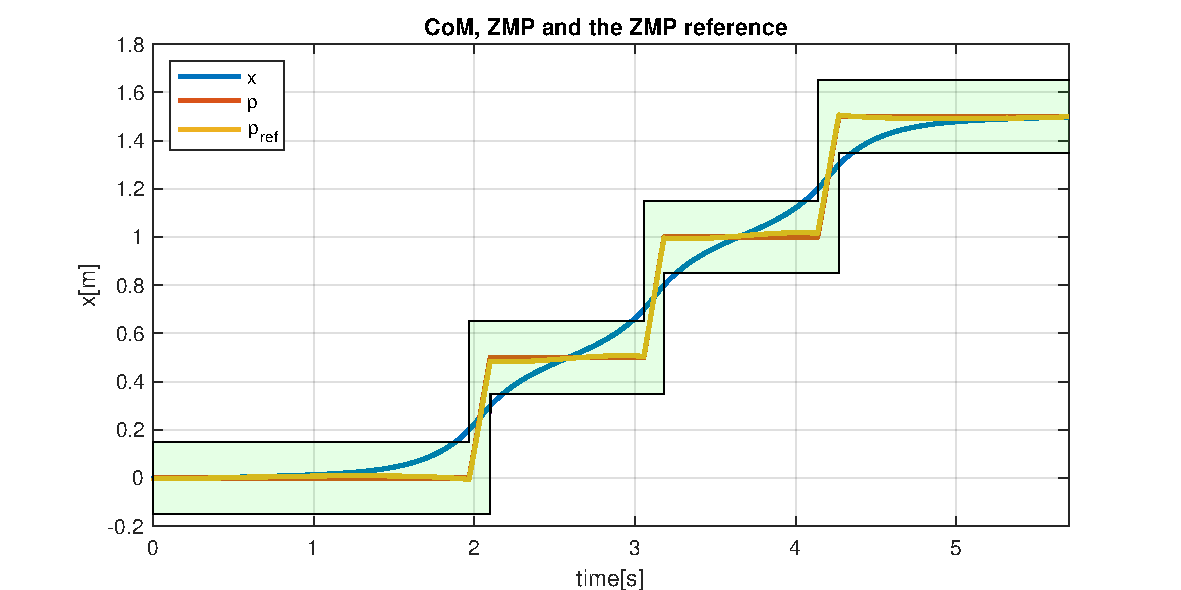
\includegraphics[scale=0.4]{plot/SQD/50/x_time_50.pdf}
        \caption{ZMP and CoM profile resulting from the optimization in time domain with $\beta=50$} 
        \label{fig:opt_x_50_time}
     \end{minipage}  
     \hfill
     \begin{minipage}[b]{0.48\textwidth}
         \centering
        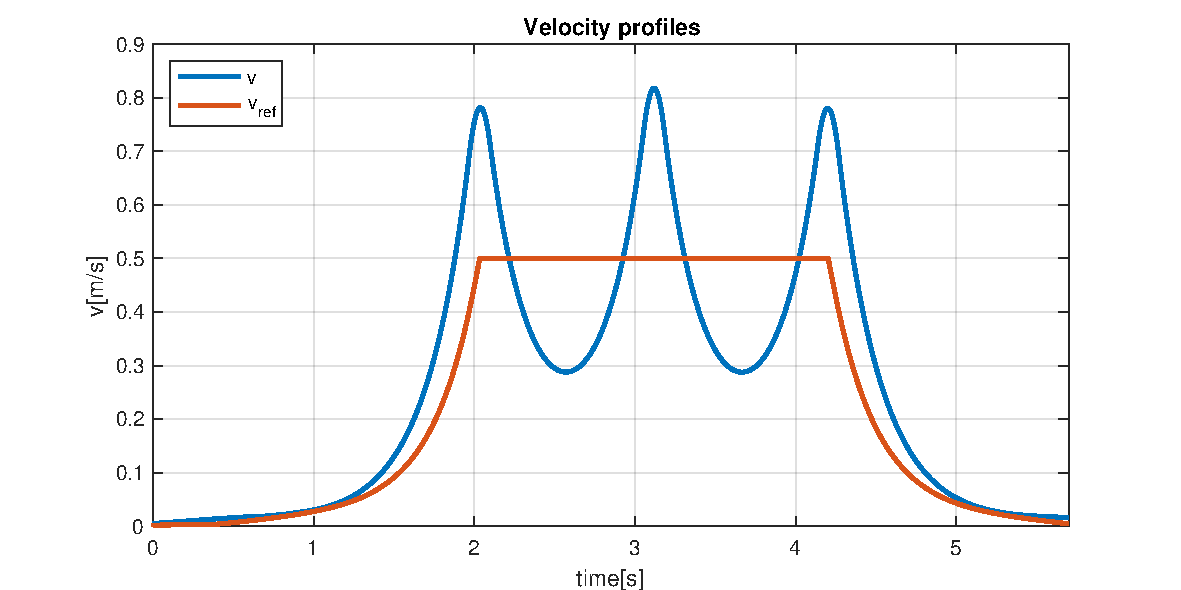
\includegraphics[scale=0.4]{plot/SQD/50/vx_time_50.pdf} 
        \caption{ZMP and CoM profile resulting from the optimization in time domain with $\beta=50$} 
        \label{fig:opt_vx_50_time}
     \end{minipage}     
    
\end{figure}

\begin{figure}

    \begin{comment}
    \begin{minipage}[b]{0.48\textwidth}
         \centering
         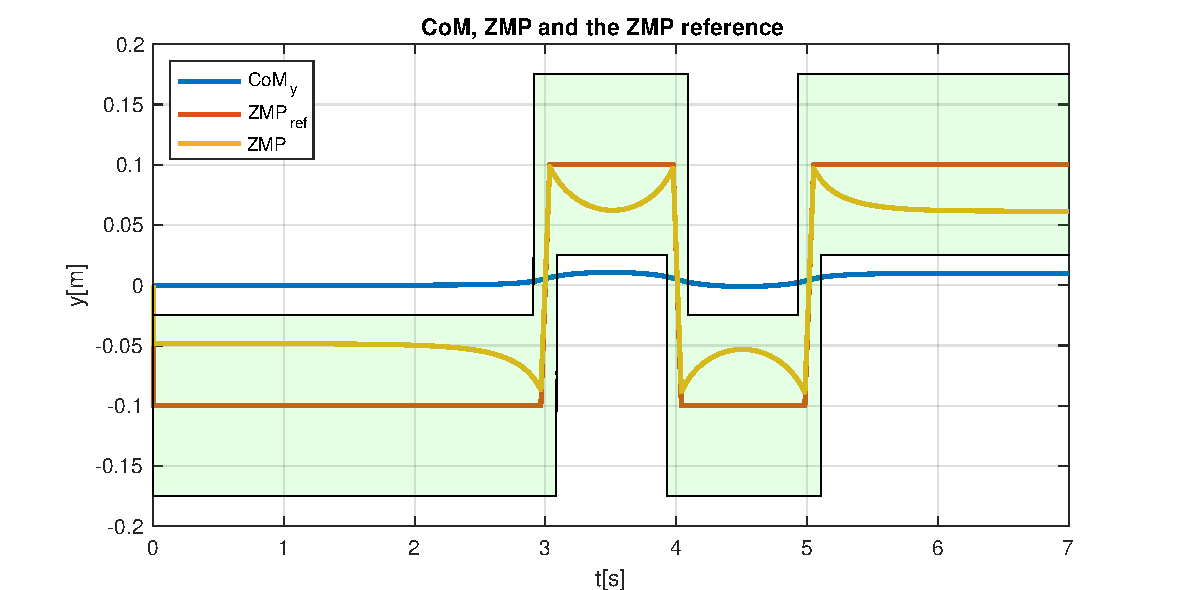
\includegraphics[scale=0.4]{plot/SQD/150/opt_y_150_time.pdf} 
         \caption{ZMP and CoM lateral motion resulting from the optimization with $\beta=1.50$ } 
         \label{fig:opt_y_150_space}
     \end{minipage}
     \hfill
     \begin{minipage}[b]{0.48\textwidth}
         \centering
        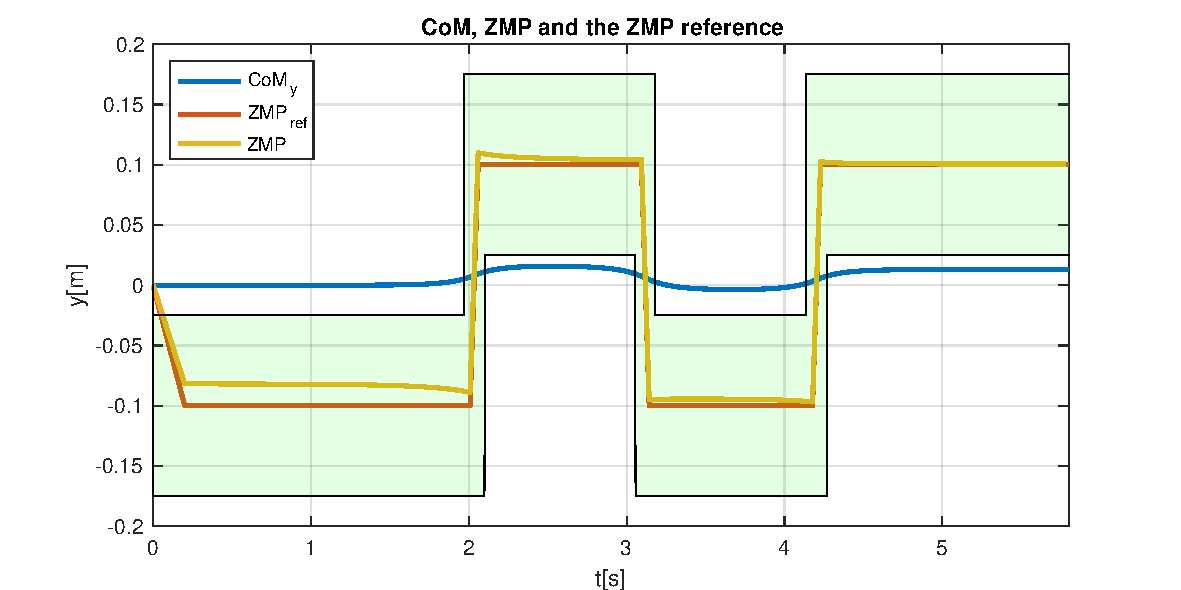
\includegraphics[scale=0.4]{plot/SQD/50/opt_y_50_time_SQD.pdf} 
        \caption{CoM speed profile lateral motion resulting from the optimization with $\beta=50$} 
        \label{fig:opt_y_50_space}
     \end{minipage}  
     \end{comment}
     \begin{minipage}[b]{0.48\textwidth}
         \centering
       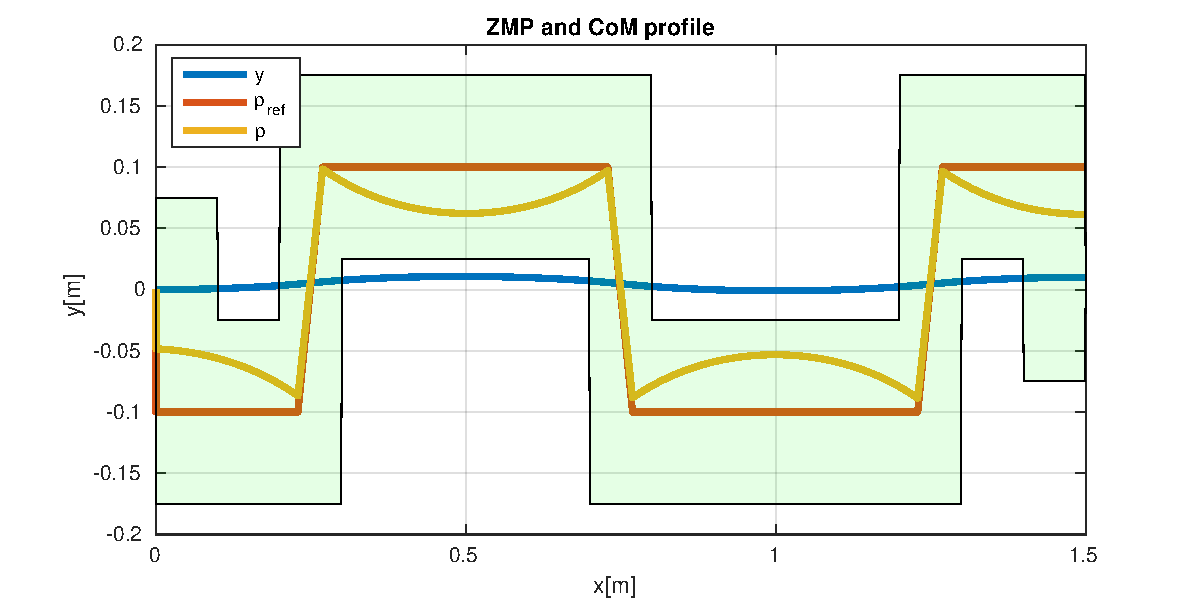
\includegraphics[scale=0.4]{plot/optimization/opt_y_150_space.pdf}
         \caption{ZMP and CoM lateral motion resulting from the optimization in space domain with $\beta=1.50$ } 
         \label{fig:opt_y_150_space}
     \end{minipage}
     \hfill
     \begin{minipage}[b]{0.48\textwidth}
         \centering
        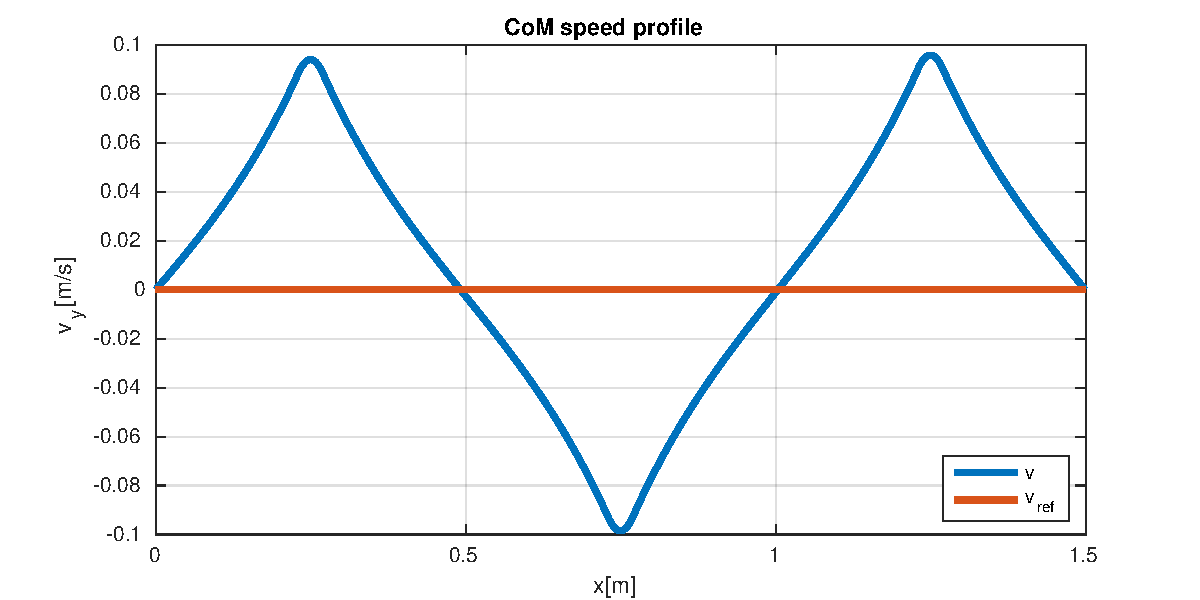
\includegraphics[scale=0.4]{plot/optimization/opt_vy_150_space.pdf}
        \caption{CoM speed profile lateral motion resulting from the optimization in space domain with $\beta=1.50$} 
        \label{fig:opt_y_50_space}
     \end{minipage} 
     \vfill
     \begin{minipage}[b]{0.48\textwidth}
         \centering
       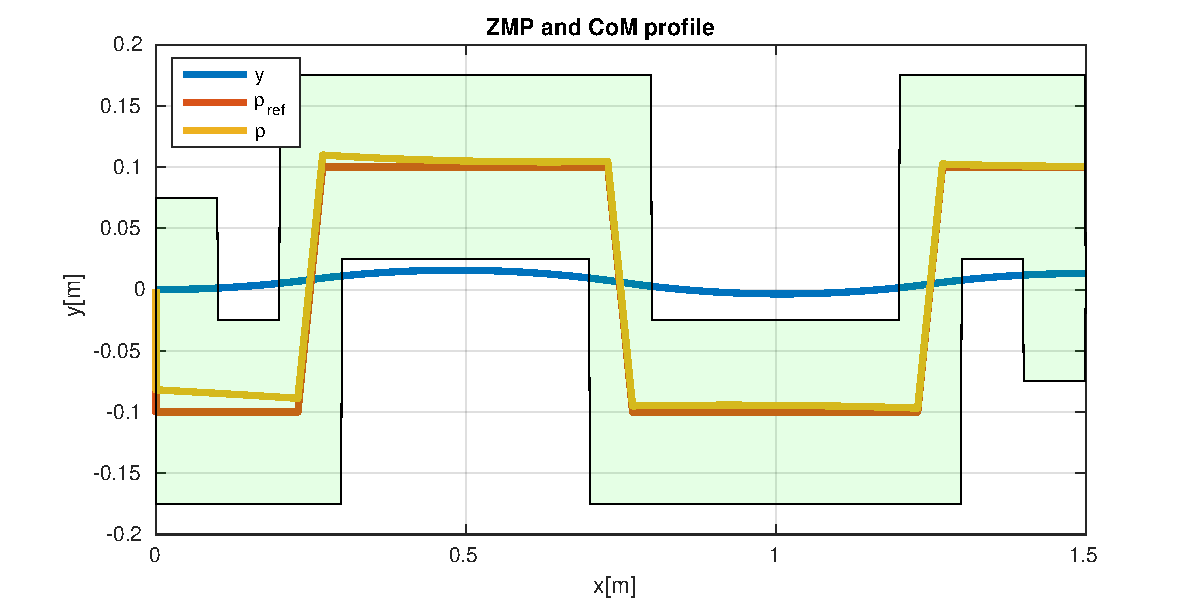
\includegraphics[scale=0.4]{plot/optimization/opt_y_50_space.pdf}
         \caption{ZMP and CoM lateral motion resulting from the optimization in space domain with $\beta=50$ } 
         \label{fig:opt_y_150_space}
     \end{minipage}
     \hfill
     \begin{minipage}[b]{0.48\textwidth}
         \centering
        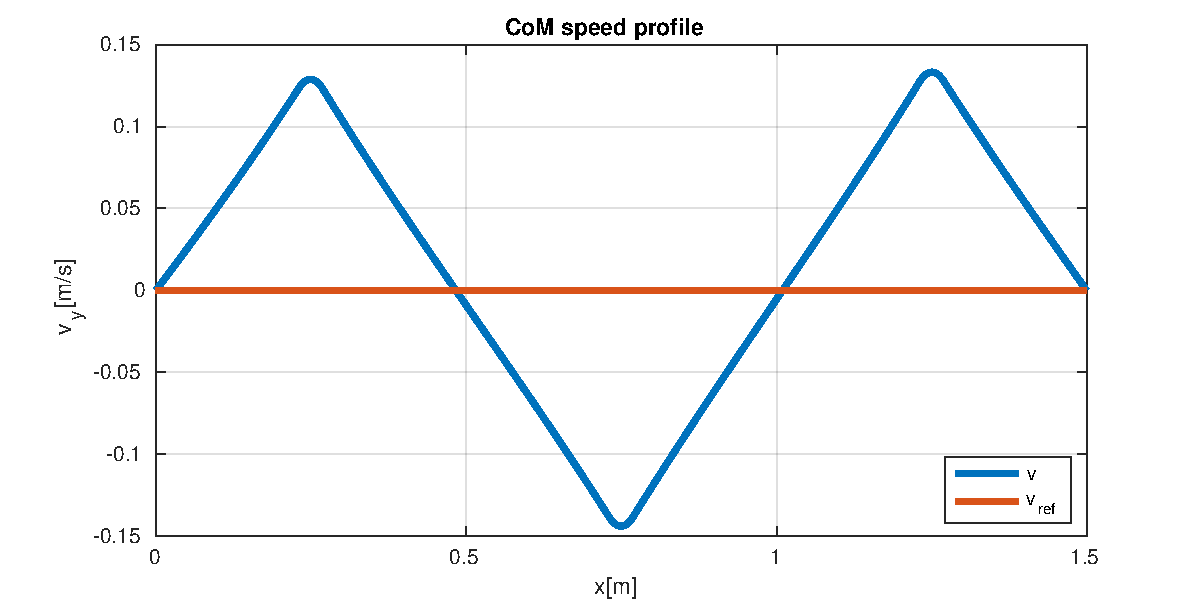
\includegraphics[scale=0.4]{plot/optimization/opt_vy_50_space.pdf}
        \caption{CoM speed profile lateral motion resulting from the optimization in space domain with $\beta=50$} 
        \label{fig:opt_y_50_space}
     \end{minipage} 
     \vfill
     \begin{minipage}[b]{0.48\textwidth}
         \centering
        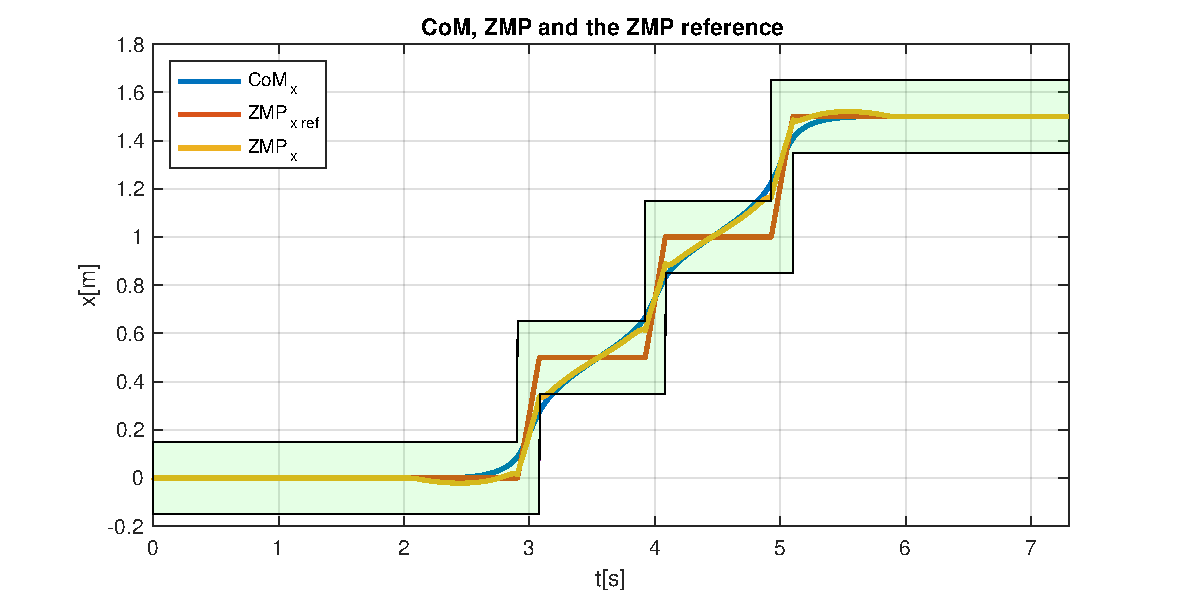
\includegraphics[scale=0.4]{plot/OPT_TEMPO/150/opt_x_150_time_noSQD.pdf} 
         \caption{ZMP and CoM profile resulting from the optimization with $\beta=1.50$} 
         \label{fig:opt_x_150_NO_SQD}
     \end{minipage}
     \hfill
     \begin{minipage}[b]{0.48\textwidth}
         \centering
        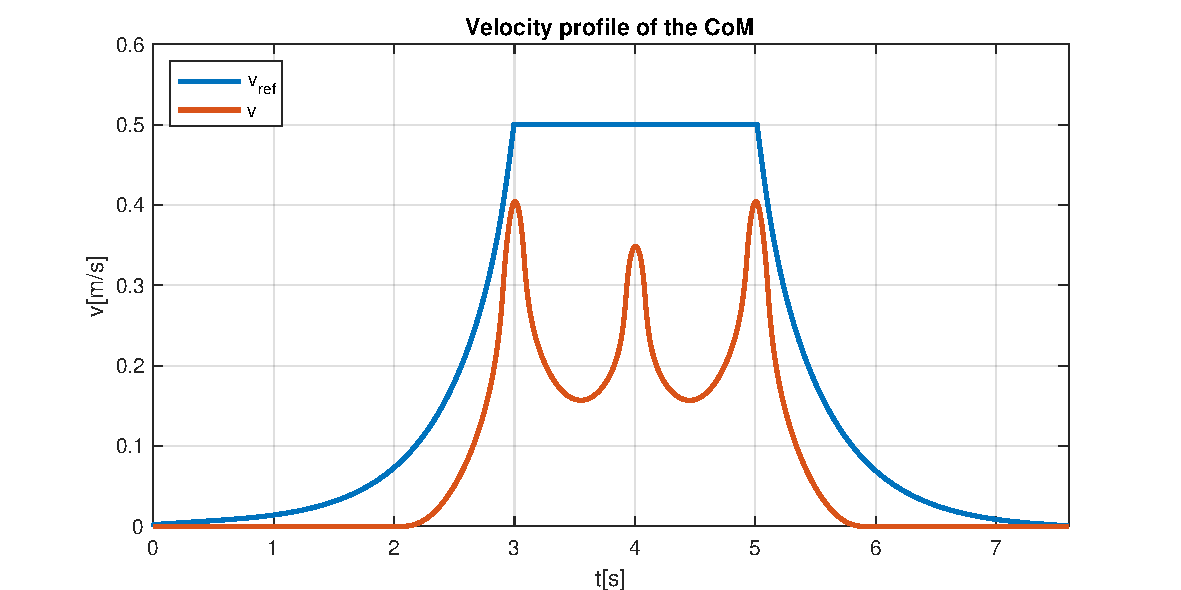
\includegraphics[scale=0.4]{plot/OPT_TEMPO/150/v_opt_x_150_time_noSQD.pdf} 
        \caption{CoM speed profile resulting from the optimization with $\beta=1.50$} 
        \label{fig:opt_vx_150_NO_SQD}
     \end{minipage}   
     \vfill
     \begin{minipage}[b]{0.48\textwidth}
         \centering
        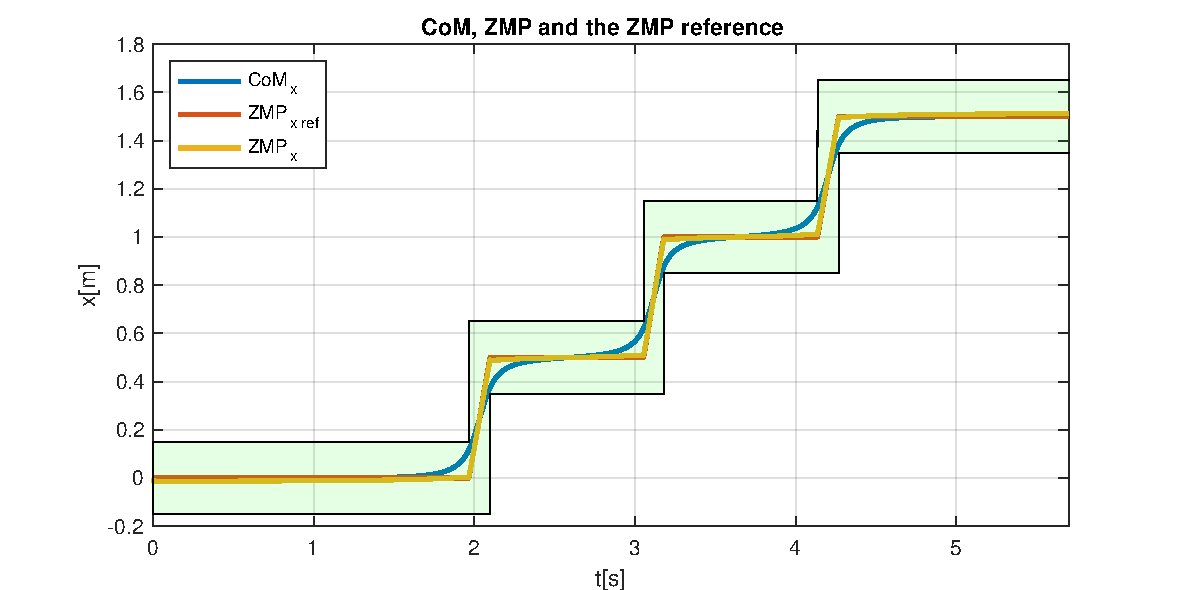
\includegraphics[scale=0.4]{plot/OPT_TEMPO/50/opt_x_50_time_noSQD.pdf}
        \caption{ZMP and CoM  profile resulting from the optimization in time domain with $\beta=50$} 
        \label{fig:opt_x_50_NO_SQD}
     \end{minipage}  
     \hfill
     \begin{minipage}[b]{0.48\textwidth}
         \centering
        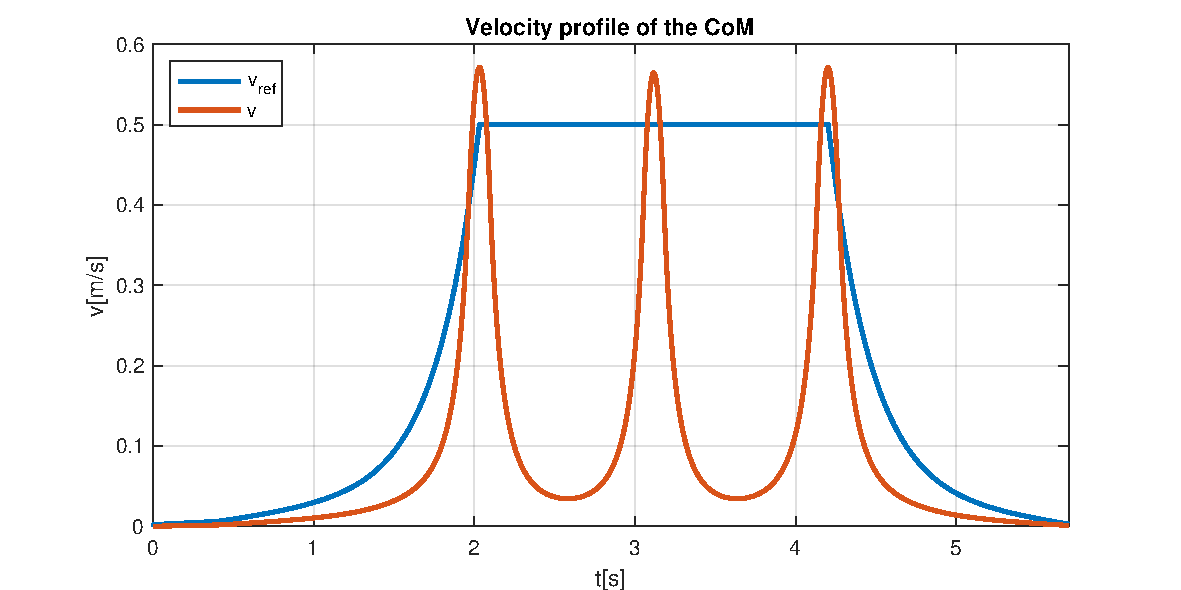
\includegraphics[scale=0.4]{plot/OPT_TEMPO/50/v_opt_x_50_time_noSQD.pdf} 
        \caption{CoM speed profile resulting from the optimization with $\beta=50$} 
        \label{fig:opt_vx_50_NO_SQD}
     \end{minipage}   

\end{figure}

\begin{figure}
 \begin{minipage}[b]{0.48\textwidth}
         \centering
         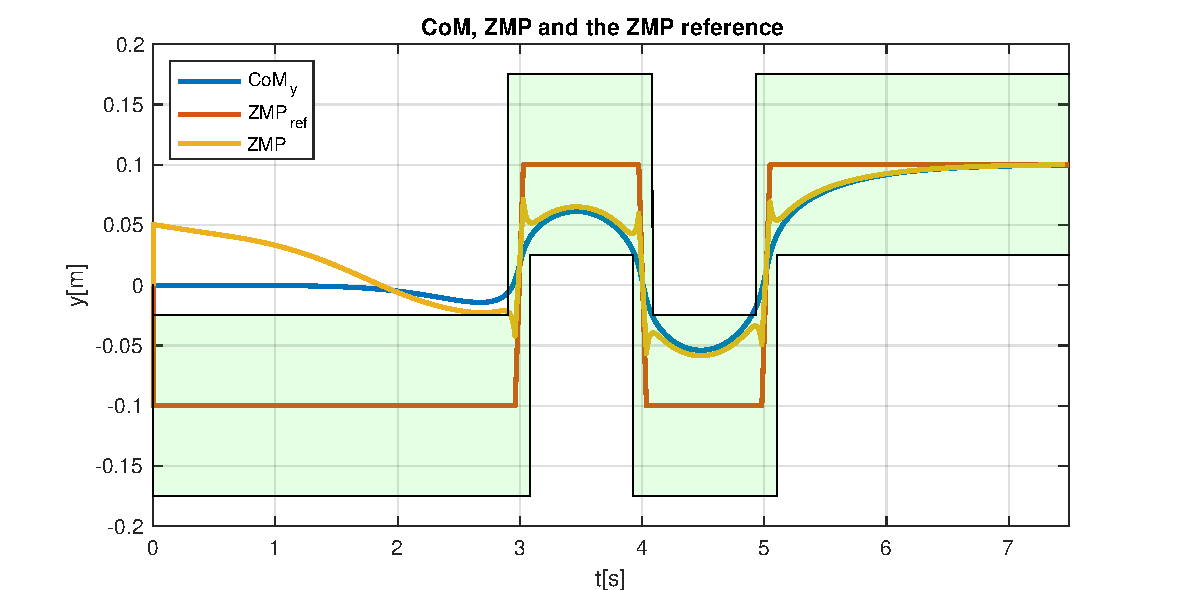
\includegraphics[scale=0.4]{plot/OPT_TEMPO/150/opt_y_150_time_noSQD.pdf} 
         \caption{ZMP and CoM lateral motion resulting from the optimization with $\beta=1.50 $} 
         \label{fig:opt_y_150_NO_SQD}
     \end{minipage}
     \hfill
     \begin{minipage}[b]{0.48\textwidth}
         \centering
        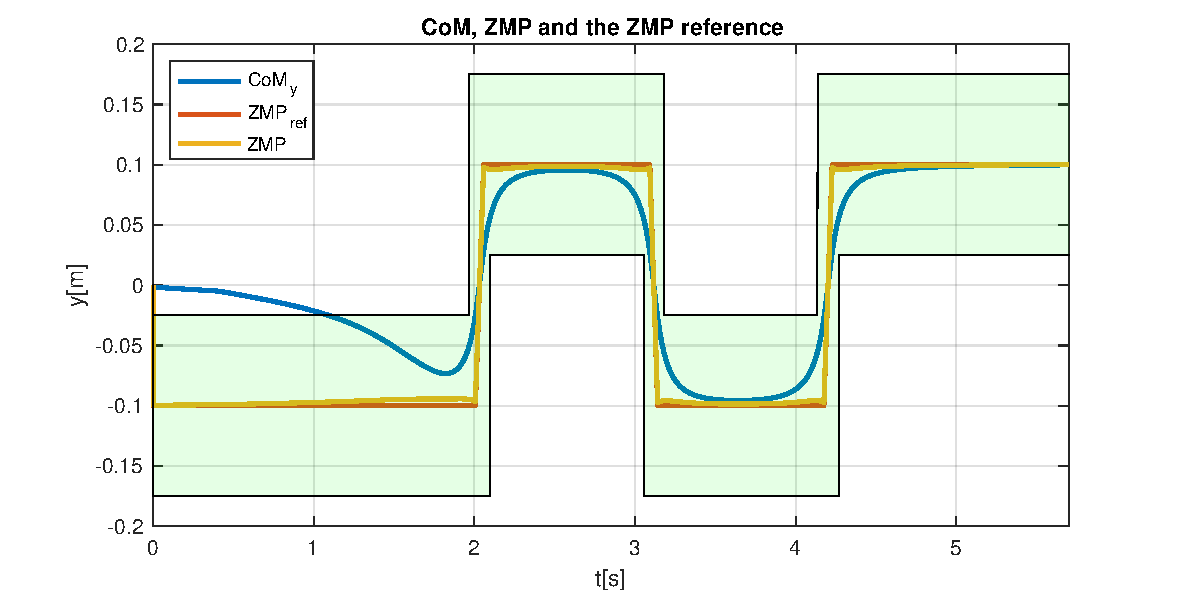
\includegraphics[scale=0.4]{plot/OPT_TEMPO/50/opt_y_50_time_noSQD.pdf} 
        \caption{CoM speed profile lateral motion resulting from the optimization with $\beta=50$} 
        \label{fig:opt_y_50_NO_SQD}
     \end{minipage}   

\end{figure}

  
\begin{figure}
         \centering
        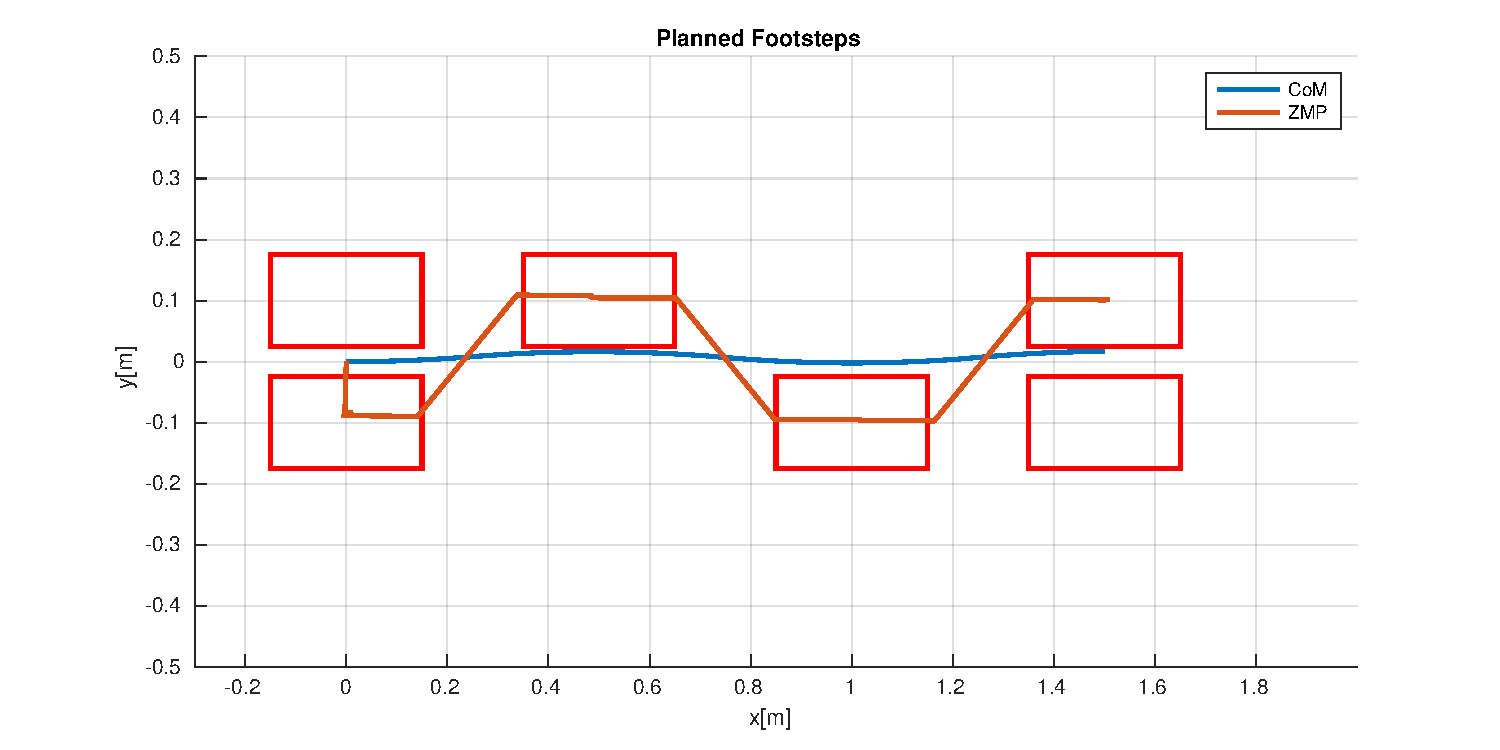
\includegraphics[scale=0.6]{plot/optimization/footsteps_com_zmp.pdf}
        \caption{Simulation of three steps with $\beta=50$} 
        \label{fig:steps_NOsqd}
\end{figure}
     



\newpage

\section{Conclusions}

In this project I have reproduced the fundamental results of the paper \cite{Kaj1}. I started from the classical optimization problem in time domain , to get the evolution of the CoM and the ZMP in time, which I later used as comparison with respect to the new method introduced in the paper on which the project is based on. Then I have formalized the same problem in the space domain by introducing the SQD, that is the LIP model discretized in the space domain, and I have solved the optimization problem along the sagittal axis, instead for the lateral motion I solved the optimization problem directly in the time domain because it is not possible to solve in the space domain. Using this kind of discretization I also transform the linear convex optimization problem into a nonlinear non-convex optimization problem. As a consequence the computation time to get the solution increased remarkably and also due to the non convexity the solution that I got may be not the optimal one, but the results are acceptable. This is the first big drawback of this new technique, in fact for how I implemented the optimization problem, i.e I  optimized on the whole horizon at once, it is not possible to use it as an online technique, but this is not a problem because it is conceived as an off line technique. After obtaining the evolution of the CoM along $x$ and $y$ axis and the evolution of the ZMP with respect to the hip position I focused on the kinematic part. The aim of the kinematic part is to find the values of the legs joints to allow the robot to walk with stretched knee, so first of all I compared three different numeric inverse kinematic algorithms that are Gradient method, Newton method and Levenberg-Marquardt method and I choose Newton method because it has better performances with respect to the other methods, and also for the reason explained at the end of section \ref{sec:KWP}. In order to tackling the problem gradually I started with a simplified leg of 3 DoF and I computed all the joint values along the path, in which I made an analogy with a manipulator, where the hip is the moving base and the heel is the end effector. In this way I have completed the the spatial walking pattern SPW, that is an array generated offline in which there are the evolution of the ZMP, the evolution of CoM velocity and the values of the joint at every discretization step expressed in the space domain. After that, I  increased the difficulty by considering the 5 DoF leg that allowed us to add the lateral motion to the robot, in fact these two extra DoFs  are two revolute joints at the hip of the robot. Once I have generated these spatial walking patterns, for the 3 DoF and for the 5 DoF I implemented a kinematic biped walker in order to visualize the results. So I defined the DH tables and the homogeneous transformation between the hip and the Matlab frame and I plotted the leg by computing the forward kinematic for reach the joints and then I linked them with a segment. Additionally I measured some performance indexes to evaluate the  inverse kinematic performance along the whole path. At the end I gave an idea on how to perform the conversion from the space domain to the time domain that is necessary to implement this method for a dynamic simulation, that I did not perform, or to implement on a real robot.\\
This new version of the biped walking generation based on the control of the ZMP has many drawbacks. The most crucial are that the optimization problem is more difficult to solve with respect to the classic case in the time domain, it is not implementable in real time because the SPW is generated offline, the discretized model is nonlinear and it has a singularity when the CoM speed is zero. The advantage is that it is more flexible, in the sense that it is possible to realize versatile gait generation and in fact I allow the robot to walk with stretched knee, instead in the classical formulation of the problem in time domain the robot walks in a crouch position due to the more conservative gait design. Even if this method add this important advantage the benefit of the SQD compared with conventional methods is still unclear.


\newpage

\begin{thebibliography}{7}
\bibitem{Kaj1} S. Kajita et al., "Biped walking pattern generation based on spatially quantized dynamics," 2017 IEEE-RAS 17th International Conference on Humanoid Robotics (Humanoids), Birmingham, UK, 2017, pp. 599-605, doi: 10.1109/HUMANOIDS.2017.8246933.
\bibitem{Vukobratovic}Vukobratovic, Miomir  Borovac, Branislav. (2004). Zero-Moment Point - Thirty Five Years of its Life.. I. J. Humanoid Robotics. 1. 157-173. 10.1142/S0219843604000083. 
\bibitem{Tassa}  Y. Tassa, N. Mansard and E. Todorov, "Control-limited differential dynamic programming," 2014 IEEE International Conference on Robotics and Automation (ICRA), Hong Kong, China, 2014, pp. 1168-1175, doi: 10.1109/ICRA.2014.6907001.
\bibitem{Kelmar}Kelmar, L.  Khosla, Pradeep. (1988). Automatic generation of kinematics for a reconfigurable modular manipulator system. 663 - 668 vol.2. 10.1109/ROBOT.1988.12135. 
\bibitem{LMmethod} T. Sugihara, "Solvability-unconcerned inverse kinematics based on Levenberg-Marquardt method with robust damping," 2009 9th IEEE-RAS International Conference on Humanoid Robots, Paris, France, 2009, pp. 555-560, doi: 10.1109/ICHR.2009.5379515.

\bibitem{mpcMatlab} Optimization Problem - MATLAB \& Simulink https://www.mathworks.com/help/mpc/ug/optimization-problem.html
\bibitem{HumanBook}S. Kajita, H. Hirukawa, K. Harada, and K. Yokoi, Introduction to Humanoid Robotics. Springer Publishing Company Inc., 2014.
\end{thebibliography} 


\end{document}